\documentclass[12pt]{article}
\usepackage[utf8]{inputenc}
\usepackage{graphicx} % Allows you to insert figures
\usepackage{amsmath} % Allows you to do equations
% \usepackage{amssymb} BREAKING LAYOUT, WILL LOOK INTO IT SOON
% AVOID SETSPACE WHICH RESETS SPACING
\usepackage{enumitem} % for list items
\usepackage{tikz}
\usetikzlibrary{calc, shapes.geometric,matrix,decorations.pathreplacing}
\usepackage[latte,styleAll]{catppuccinpalette}
\usepackage{float} % for \begin{figure}[H]
\usepackage{caption}
\usepackage[english]{babel}
\usepackage{csquotes, lipsum, ragged2e}
\usepackage[dvipsnames]{xcolor}
\usepackage[backend=bibtex, language=auto, autolang=other, bibencoding=utf8]{biblatex}
\usepackage{fontspec}
\usepackage{xstring}
\usepackage{geometry} % Formats the paper size, orientation, and margins

\geometry{
 a4paper,
 left=20mm,
 top=20mm,
 }

\setlength{\parskip}{1em} % paragraphs separated by one line
\usepackage[format=plain,
            font=it]{caption} % Italicizes figure captions
\setsansfont{P052}[
    Path=./fonts/palladio/,
    Scale=0.85,
    Extension = .ttf,
    UprightFont=*-Roman,
    BoldFont=*-Bold,
    ItalicFont=*-Italic,
    BoldItalicFont=*-BoldItalic
]
\setmonofont{IBMPlexMono}[
    Path=./fonts/IBMPlex/,
    Scale=0.85,
    Extension = .ttf,
    UprightFont=*-Regular,
    BoldFont=*-Bold,
    ItalicFont=*-Italic,
    BoldItalicFont=*-BoldItalic
    ]
\newfontfamily\virgil{Virgil}[
    Path=./fonts/,
    Extension=.ttf % Change to .otf if applicable
]
% SET GLOBAL DEFAULT FAMILY
\renewcommand{\familydefault}{\sfdefault}
% SET GLOBAL DEFAULT FAMILY
% \usepackage[T1]{fontenc}
% \usepackage{tgbonum}
% https://www.overleaf.com/learn/latex/Font_typefaces
\definecolor{kwcolor}{rgb}{0.902,0.75,0.478}
\definecolor{sblue}{HTML}{C1E8F7}
\definecolor{syellow}{HTML}{F1F4C1}
\definecolor{sorange}{HTML}{FFE2BB}
\definecolor{sstart}{HTML}{FBE0E0}
\definecolor{sgreen}{HTML}{CCE7CF}
\definecolor{spurple}{HTML}{C5BEDE}

\definecolor{BasePythonColor}{HTML}{C678DC}
\usepackage{listings}
\lstdefinestyle{python}{
  backgroundcolor=\color[rgb]{0.91,0.925,0.929},
  language={python},
  breaklines=true,
  showstringspaces=false,
  breakatwhitespace=true,
  stringstyle = {\color{CtpGreen}},
  commentstyle={\color{CtpOverlay1}},
  basicstyle = {\small\color{CtpText}\ttfamily},
  keywordstyle = {\color{CtpMauve}},
  keywordstyle = [2]{\color{CtpBlue}},
  keywordstyle = [3]{\color{CtpBlue}},
  keywordstyle = [4]{\color{CtpLavender}},
  keywordstyle = [5]{\color{CtpPeach}},
  keywordstyle = [6]{\color{CtpTeal}},
  otherkeywords = {<, ||, =, ?},
  morekeywords = [2]{import, if, def, repr},
  morekeywords = [3]{Model, forward, all, format, nn, functional, nn.Module},
  morekeywords = [4]{@page},
  morekeywords = [5]{exception, do_some_for_pages, @page, @admin},
  morekeywords = [6]{<, ||, =, ?},
  framexleftmargin=3pt,
  framextopmargin=1pt,
  framexbottommargin=1pt, 
  frame=tb, framerule=0pt,
}

\lstdefinestyle{C}{
    belowcaptionskip=1\baselineskip,
    breaklines=true,
    numbers=none, 
    basicstyle=\footnotesize\ttfamily,
    keywordstyle=\bfseries\color{green!40!black},
    commentstyle=\itshape\color{purple!40!black},
    identifierstyle=\color{blue},
    backgroundcolor=\color[rgb]{0.91,0.925,0.929},
    framexleftmargin=1pt,
    framextopmargin=1pt,
    framexbottommargin=1pt, 
    frame=tb, framerule=0pt,
    showstringspaces=false
}
\definecolor{xsocial}{HTML}{1C9BEF}
\definecolor{xtitle}{HTML}{1E6A41}
\definecolor{xlink}{HTML}{036EE8}
% Define a custom command
\newcommand{\customtext}[3]{% 
    \vspace{#2} % #2 is the vertical spacing
    \fontsize{13}{8}\textcolor{#1}{\textit{#3}}% #1 is the color, #3 is the text
}
\newcommand{\bandi}[1]{\textbf{\textit{#1}}}
% \newcommand{\sidecite}[1]{\scriptsize\ \textcolor{blue}{$ \mathbf{^{#1}}$}\normalsize}
\newcommand{\sidecite}[1]{\textsuperscript{\textcolor{blue}{\textbf{\scriptsize#1}}}}
\newcommand{\customtitle}[1]{\fontsize{14}{8}\textcolor{xtitle}{\textit{#1}}\\}
\newcommand{\itred}[1]{\scriptsize \textcolor{red}{\it #1}}
\newcommand{\imagebullet}{$\vcenter{\hbox{\includegraphics[width=0.4cm]{images/modal.png}}}$}
\newcommand{\maincitecount}{\sidecite{\stepcounter{maincite}\themaincite}}
\newcommand{\sidecitecount}{$^{\stepcounter{sidecite}\thesidecite}$}

\usepackage{hyperref}
\hypersetup{
    colorlinks=true,
    linkcolor=xlink,
    filecolor=xlink,      
    urlcolor=xlink,
    pdftitle={Overleaf Example},
    pdfpagemode=FullScreen,
}

\urlstyle{same}
\usepackage{fontawesome}
\begin{document}
\include{codesintikz.tex}
\linespread{1.2}\selectfont
\title{GPGPU Programming with CUDA}
\author{Marvin}
\date{\today}

% sidecite counter
\newcounter{maincite}
\newcounter{sidecite}
% \maketitle
% PAGE 1

\begin{figure}[!htb]
    \begin{minipage}[t]{0.65\textwidth}
    {\sffamily 
    \fontsize{21}{8}\textcolor{xtitle}{\textit{Scaling ViTs across Training Compute}}\\
    \fontsize{9}{8}\textcolor{xtitle}{
        \textit{
            \ by \href{https://www.linkedin.com/in/marvin-mboya}{Marvin Mboya\ \faLinkedinSquare}
    }}\\
    }\\
    [-0.3cm]
    \textcolor{xtitle}{{\it A journey across optimization levels}}\\
    [0.2cm]
    \normalsize
    \raggedright
    Looking back at when we could only reliably produce Shakespearean poetry with {\it RNNs}, a thin line between hallucinations 
    and poetry, one can see why Google open sourcing Transformers was the just needed {\it krabby patty secret formula} to SOTA 
    models toppling leaderboards every coming week, and copyright lawsuits enriching the lawyers in the same way that AI ideas 
    could be well thought out as a well pipelined autocomplete service driving some startups.\\ 
    % Too bad {\it Plankton} lives under the sea!\\
    This article is a no exception, {\it thanks Transformers!}, written from the curiosity that inspires I to 
    sit on the shoulders of giants, intellectually speaking, and start off this chain of optimization across languages and hardware 
    stack that only climaxes limited to the largest GPU compute I can access without feeling like I have leaked my AWS cloud keys 
    to the best crypto miners in the east continents!
    \vspace{1.5em}\\
    \fontsize{14}{8}\textcolor{xtitle}{\textit{Back in time}}\\
    {\it Vaswani et al.} didn't understand the gravity of their research{\maincitecount} when they lightly ended their paper, but 
    it inspired to generalize learning in the natural language domain, being largely parallelizable and solving saturation in 
    training performance for increased training data.\\
    Recurrent Neural Networks{\maincitecount} was the precursor to this, its encoder that generates the latent space representation of the input tokens
    working in such a way that it captures the entire meaning of the input sentence in its final hiddetn state. This processing of the 
    entire input text was its drawback as it could not access intermediate hidden states hence not capturing dependencies within words
    in the sentence.\\
    \vspace{1em}
    \small \textcolor{xtitle}{\textbf{\textit{Sweet sauce of Transformers}}}\\
    \normalsize
    Parallelizability, scaled dot product attention, and scaling of models to unprecedented size while maintaining trainability.
    
    \end{minipage}
    \hspace{25pt}
    \begin{minipage}[t]{.4\textwidth}
      \raggedright
      \scriptsize 
      {\sidecitecount} \href{https://arxiv.org/abs/1706.03762}{arXiv:1706.03762}\\
      {\it Attention is all you need}\\
      {\it Vaswani et al. 2017}\\
      \vspace{2em}
      {\sidecitecount} RNNs can be understood using a special key word, {\it \bf recurrent}, meaning to recur, where each hidden 
      state would have a loop within itself and also includes the compounded outputs of all the previous hidden states,
      hugely based on the concept of a Markov model\\
      \vspace{2em}
      {\bf Markov process} is a stochastic process with the properties:
      \begin{itemize}[left=0pt,topsep=0pt,itemsep=-1ex,parsep=0ex]
        \item number of posssible states is finite
        \item outcome at any state depends only on outcomes pf previous states
        \item probabilities are constant over time 
      \end{itemize}
      where a \textit{\textbf{stochastic process}} can be said as a probability distribution over a space of paths;
      this path often describing the evolution of some {\bf random variable} over time.\\
      \vspace{1em}
      A random variable, despite its name, is never random, and not a variable, it is a deterministic function.\\
      \vspace{1em}
      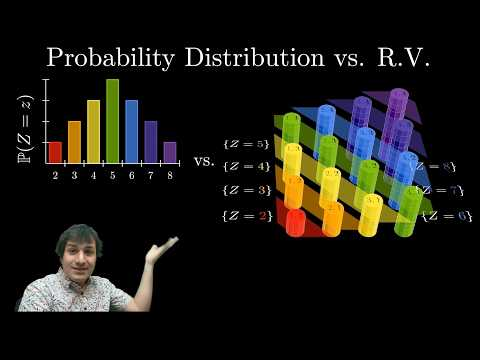
\includegraphics[width=0.5\textwidth]{images/rvnotrandom.jpg}\\
      Thanks to Dr Mihai for this awesome video explaining much on this
      \tiny \url{https://youtu.be/KQHfOZHNZ3k?si=jWPeMLZV0EF76mGz}
    \end{minipage}
\end{figure}
\pagebreak
% PAGE 2
\begin{figure}[!htb]
    \begin{minipage}[t]{0.65\textwidth}
    \raggedright
    \customtext{xtitle}{0em}{From a black box approach}\\
    Given a text {\small \textit{\textbf{The ruler of a kingdom is a}}} with the next likely word 
    being \textit{\textbf{\small king}}, humanly thinking, how is the input sentence then passed to a 
    Transformers model?\\ 
    Basically, computational models cannot process strings, hence it needs conversion to a vector of integers, each word (or subword) 
    uniquely mapped to a corresponding integer, a process known as {\it tokenization}. A basic form 
    would be a hashmap of words to integers and vice versa for getting a word from index of maximum 
    probability in softmaxed one-dimensional distribution of output float values {\maincitecount}.\\
    \vspace{0.5em}
    Implementing a simple tokenizer based on the vocabulary{\maincitecount} we have, 
\begin{lstlisting}[language=python,style=python,,basicstyle=\ttfamily\footnotesize]
text = "The ruler of a kingdom is a"
text = text.lower() # making tokenizer case insensitive 
text = text.split() # getting individual words 
# as separated by spaces 
vocab = list(sorted(set(text)))
words_to_ids = {word:i for i, word in enumerate(vocab)}
ids_to_words = {v:k for k,v in words_to_ids.items()}
\end{lstlisting}
Great, now we have lookup tables (the last two lines), and a naive preprocessing of text needed 
before tokenization.  So then, let's tokenize \textcolor{xtitle}{the kingdom had another ruler}.
Wait?! The lookup table does not have the words \textcolor{xtitle}{"another", "had", "another"}! 
Let's improve it so any word not part of the original vocabulary be assigned a new unique id{\maincitecount}.
\begin{lstlisting}[language=python,style=python,,basicstyle=\ttfamily\footnotesize]
words_to_ids = {word:i for i, word in enumerate(vocab)}
ids_to_words = {v:k for k,v in words_to_ids.items()}
def lookup(word):
    try: 
        id = words_to_ids[word]
    except KeyError:
        vocab.append(word)
        words_to_ids[word] = len(vocab) - 1
        ids_to_words[len(vocab)-1] = word 
        id = words_to_ids[word]
    return id 
\end{lstlisting}
    \end{minipage}%
    \hspace{25pt}
    \begin{minipage}[t]{.4\textwidth}
      \raggedright
      \scriptsize 
      {\sidecitecount} the commonly used tokenizer is tiktoken, using a concept called Byte-Pair Encoding to 
      map subwords to ids using a look-up table that takes into account frequencies of subwords.\\
      \vspace{2em}
      {\sidecitecount} vocabulary {\tiny $\sim$} set of unique words (or subwords based on the tokenization strategy) 
      in all words of the entire training dataset used to train a particular large language model.\\
      \vspace{2em}
      {\sidecitecount} our look-up tables are very much capable of any encoding and decoding (for the tiny tiny vocabulary).
    \end{minipage}
\end{figure}
% PAGE 3
\pagebreak
\begin{figure}[!htb]
    \begin{minipage}[t]{0.65\textwidth}
    \raggedright
    \customtext{xtitle}{0em}{Trying our shiny code}\\
\begin{lstlisting}[language=python,style=python,,basicstyle=\ttfamily\footnotesize]
sentence = "the kingdom had another ruler"
tokens = [lookup(word) for word in sentence.lower().split()]
print(tokens)
# [5, 2, 6, 7, 4]
words_gotten = [ids_to_words[id] for id in tokens]
sentence_gotten = " ".join(words_gotten)
print(sentence_gotten)
# "the kingdom had another ruler"
\end{lstlisting}
\textbf{\textit{\small Note}} that the above implementation of tokenization is to help you understand a baseline of what happens 
under the hood in conversion of what models cannot deal with, strings, to a format that can be computationally 
crunched.\\
Hoever, when looking into the Transformers model architecture as outlined in the paper\sidecite{1}, also in{\maincitecount}
for convenience, it is seen that the first block is an Embedding block.\\
\customtext{xtitle}{1em}{What about the Embeddings block?}\\
Well, the vector of integers as input in itself cannot capture rich latent representations of the input tokens, 
so the Embeddings block{\maincitecount} does just that, mapping the tokens to higher dimensions. The embeddings block is usually 
\bandi{V} by \bandi{D}, where \bandi{V} is the size of the vocabulary, and \bandi{D} is an abstract dimension of your choosing, 
the higher the better, but more computationally expensive and longer to process.\\
Using PyTorch, an Embeddings block of {\it D being 3} can be implemented as:
\begin{lstlisting}[language=python,style=python,,basicstyle=\ttfamily\footnotesize]
import torch, torch.nn as nn 
V, D = len(vocab), 3
emb = nn.Embedding(V,D)
higher_emb_tokens = emb(torch.tensor(tokens))
print(higher_emb_tokens.shape) # torch.Size([5, 3])
\end{lstlisting}
One of the best LLMs ever open sourced by Meta, the Llama 3, the 3 billion parameter size variant, has its vocabulary with {\it 128K} tokens.
and the embedding dimensions, \bandi{D}, being 3072.
    \end{minipage}%
    \hspace{25pt}
    \begin{minipage}[t]{.4\textwidth}
      \raggedright
      \scriptsize 
      {\sidecitecount} Transformers architecture\\
      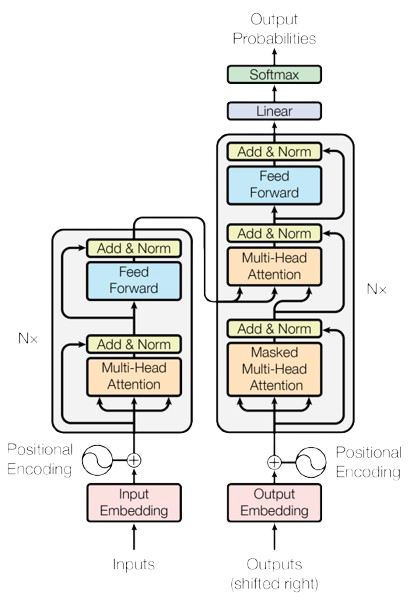
\includegraphics[width=\textwidth]{images/transformers.png}\\
      \vspace{2em}
      {\sidecitecount} {\it nn.Embedding} is just {\it nn.Linear} but only that {\it nn.Embedding} simplifies retrieving rows from its weights 
      such that you don't pass it one hot vectors but just indeces basically same as the position of the single {\it 1s} in the 
      one-hot vector you would have passed to {\it nn.Linear}
    \end{minipage}
\end{figure}
\pagebreak
% PAGE 4
\begin{figure}[!htb]
    \begin{minipage}[t]{0.65\textwidth}
    \raggedright
    \customtext{xtitle}{0em}{Positional Encoding}\\
    Before the Multi-Head Attention (MHA) block, the positional encoding is attached to the graph to constitute the position information and 
    this allows the model to easily attend to relative positions.
    Why is that? Well, the MHA block is permutation-equivariant, and cannot distinguish whether an input comes before another one in the 
    sequence or not.\\
    The meaning of a sentence can change if words are reordered, so this technique retains information about the order of the words in a sequence.\\
    Positional encoding is the scheme through which the knowledge of the order of objects in a sequence is maintained.\\
    This post by Christopher{\maincitecount} highlights the evolution of positional encoding in transformer models, a worthy read! For this article, 
    let's focus on the rotary positional embedding (RoPE){\maincitecount}.\\    
    % \vspace{0.5em}
    % \customtext{xtitle}{1em}{Why this encoding?}\\
    % Previous approaches to encoding did first incorporate positional information to the context representations before transforming them to queries, keys and values. 
    % Why is this not good? Well, for linear self-attention architecture, this bias disrupts low-rank factorization hence forcing 
    % explicit computation of the position bias matrix.
    Let's making a few things clear, 
    \begin{itemize}[left=0pt,topsep=0pt,itemsep=-1ex,parsep=0ex]
        \item previous position encodings were done before the MHA block, this is done within it.
        \item RoPE is only applied to the queries and the keys, not the values. 
        \item RoPE is only applied after the vectors $\vec{q}$ and $\vec{k}$ have been multiplied by the 
        \bandi{W} matrix in the attention mechanism, while in the vanilla transformer they're applied before.
      \end{itemize}
    \vspace{1em}
    The general form of the proposed approach for RoPE is as in page 5 for a sparse matrix with pre-defined 
    parameters $\Theta=\{\theta_i=10000^{-2(i-1)/d}, i\in[1,2,...,d/2]\}$\\
    which can be implemented in code as 
\begin{lstlisting}[language=python,style=python,,basicstyle=\ttfamily\footnotesize]
assert d % 2 == 0, "dim must be divisible by 2"
i_s = torch.arange(0,d,2).float()
theta_s = 10000 ** (- i_s / d).to(device)
\end{lstlisting}
where {\it device} is code that chooses the compute device.
\begin{lstlisting}[language=python,style=python,,basicstyle=\ttfamily\footnotesize]
device = torch.device(
    "cuda" if torch.cuda.is_available() else (
    "mps" if torch.backends.mps.is_available() else "cpu"
    )
)    
\end{lstlisting}
   \end{minipage}%
    \hspace{25pt}
    \begin{minipage}[t]{.4\textwidth}
      \raggedright
      \scriptsize 
      {\sidecitecount} \scriptsize{\url{https://huggingface.co/blog/designing-positional-encoding}}\\
      \scriptsize 
      { \it You could have designed state of the art positional encoding}\\
      {\it Christopher Fleetwood}\\
      \vspace{2em}
      {\sidecitecount} 	\href{https://arxiv.org/pdf/2104.09864}{arXiv:2104.09864}\\
      {\it RoFormer: Enhanced Transformer with Rotary Position Embedding}\\
      {\it Su et al. 2022}\\
      \vspace{2em}
    \end{minipage}
\end{figure}
% PAGE 5
\pagebreak
\begin{figure}[!htb]
    \begin{minipage}[t]{0.65\textwidth}
    \raggedright
    Given the computational efficient realization which is what we're aiming at getting 
    \begin{equation*}
        \resizebox{.75\hsize}{!}{$
        \boldsymbol{R}_{\Theta,m}^d\boldsymbol{x}=
        \begin{pmatrix}
            x_1\\
            x_2\\
            x_3\\
            x_4\\
            \vdots\\
            x_{d-1}\\
            x_d
        \end{pmatrix} 
        \otimes
        \begin{pmatrix}
            \cos m\theta_1\\
            \cos m\theta_1\\
            \cos m\theta_2\\
            \cos m\theta_2\\
            \vdots\\
            \cos m\theta_{d/2}\\
            \cos m\theta_{d/2}\\
        \end{pmatrix}
        +
        \begin{pmatrix}
            -x_2\\
            x_1\\
            -x_4\\
            x_3\\
            \vdots\\
            -x_d\\
            x_{d-1}
        \end{pmatrix} 
        \otimes
        \begin{pmatrix}
            \sin m\theta_1\\
            \sin m\theta_1\\
            \sin m\theta_2\\
            \sin m\theta_2\\
            \vdots\\
            \sin m\theta_{d/2}\\
            \sin m\theta_{d/2}\\
        \end{pmatrix}
        $}
    \end{equation*}
    Having implemented $\vec{\theta}$, next let's implement {\it $m\vec{\theta}$} by way 
    of an outer product{\maincitecount}\\
\begin{lstlisting}[language=python,style=python,,basicstyle=\ttfamily\footnotesize]
m = torch.arange(context_len, device=device)
freqs = torch.outer(m, theta_s).float()    
\end{lstlisting}
\begin{equation*}
    \resizebox{.8\hsize}{!}{$
    m\vec{\theta}={\text{freqs}}=
    \begin{pmatrix}
      m_1\theta_1, m_1\theta_2, \ldots, m_1\theta_{d/2-1}, m_1\theta_{d/2}\\
      m_2\theta_1, m_2\theta_2, \ldots, m_2\theta_{d/2-1}, m_2\theta_{d/2}\\
      \vdots\hspace{2.5em}\vdots\hspace{2em}\ldots\hspace{2em}\vdots\hspace{2.5em}\vdots\\
      m_{\text{ctx\_len}}\theta_1, m_{\text{ctx\_len}-1}\theta_2,\ldots, m_{\text{ctx\_len}-1}\theta_{d/2-1}, m_{\text{ctx\_len}-1}\theta_{d/2}\\
    \end{pmatrix}
    $}
\end{equation*}
It is then needed to get the complex numbers for the resulting matrix of size context len by $d/2$.
\begin{lstlisting}[language=python,style=python,,basicstyle=\ttfamily\footnotesize]
freqs_complex = torch.polar(torch.ones_like(freqs),freqs)
\end{lstlisting}
which then gives the polar form of each element in the matrix, such that 
\begin{equation*}
    \resizebox{1.1\hsize}{!}{$
    e^{im\vec{\theta}}=
    \begin{pmatrix}
        \cos(m_1\theta_1)+i\sin(m_1\theta_1), \cos(m_1\theta_2)+i\sin(m_1\theta_2),\ldots,\cos(m_1\theta_{d/2})+i\sin(m_1\theta_{d/2})\\
        \cos(m_2\theta_1)+i\sin(m_2\theta_1), \cos(m_2\theta_2)+i\sin(m_2\theta_2),\ldots,\cos(m_2\theta_{d/2})+i\sin(m_2\theta_{d/2})\\
        \vdots\hspace{8em}\vdots\hspace{8em}\ldots\hspace{8em}\vdots\hspace{8em}\vdots\\
        \cos(m_{cl}\theta_1)+i\sin(m_{cl}\theta_1), \cos(m_{cl}\theta_2)+i\sin(m_{cl}\theta_2),\ldots,\cos(m_{cl}\theta_{d/2})+i\sin(m_{cl}\theta_{d/2})\\
    \end{pmatrix}
    $}
\end{equation*}
Let's consider a subset of the inputs and a subset of the matrix above, then\\
\vspace{-2.5em}
\begin{equation*}
    \resizebox{0.95\hsize}{!}{$
    \begin{aligned}
    \vec{x}=& \begin{pmatrix}
        x_1\\x_2\\x_3\\x_4
    \end{pmatrix}
    = \begin{pmatrix}
        (x_1\hspace{2em}x_2)\\(x_3\hspace{2em}x_4)
    \end{pmatrix}
    = \begin{pmatrix}
        x_1+ix_2\\x_3+ix_4
    \end{pmatrix}
    \otimes
    \begin{pmatrix}
        f_{11} + i\hat{f}_{11}\\
        f_{12} + i\hat{f}_{12}
    \end{pmatrix}
    \text{,\ where} 
    \begin{cases}
        f_{11} = \cos(m_1\theta_1)\\
        \hat{f}_{11}=\sin(m_1\theta_1)\\
        f_{12} = \cos(m_1\theta_2)\\
        \hat{f}_{12}=\sin(m_1\theta_2)\\
    \end{cases}\\
    =\ & (x_1 + ix_2)(f_{11} + i\hat{f}_{11})\ =\ x_1f_{11}-x_2\hat{f}_{11}+i(x_1\hat{f}_{11}+x_2f_{11})\\
    & \text{meaning} 
    \begin{pmatrix}
        x_1+ix_2\\x_3+ix_4
    \end{pmatrix}
    \otimes
    \begin{pmatrix}
        f_{11} + i\hat{f}_{11}\\
        f_{12} + i\hat{f}_{12}
    \end{pmatrix}\\
    = &
    \begin{pmatrix}
        x_1f_{11}-x_2\hat{f}_{11}+i(x_1\hat{f}_{11}+x_2f_{11})\\
        x_3f_{12}-x_4\hat{f}_{12}+i(x_3\hat{f}_{12}+x_4f_{12})\\
    \end{pmatrix} = 
    \begin{pmatrix}
        (x_1f_{11}-x_2\hat{f}_{11} \hspace{2em} x_1\hat{f}_{11}+x_2f_{11})\\
        (x_3f_{12}-x_4\hat{f}_{12} \hspace{2em} x_3\hat{f}_{12}+x_4f_{12})\\
    \end{pmatrix}\\
    & \text{rearranging gives}\\
    = &
    \begin{pmatrix}
        x_1f_{11}-x_2\hat{f}_{11}\\
        x_1\hat{f}_{11}+x_2f_{11}\\
        x_3f_{12}-x_4\hat{f}_{12}\\
        x_3\hat{f}_{12}+x_4f_{12}\\
    \end{pmatrix}
    \Rightarrow
    \begin{pmatrix}
        x_1\cos m_1\theta_1-x_2\sin m_1\theta_1\\
        x_1\sin m_1\theta_1+x_2\cos m_1\theta_1\\
        x_3\cos m_1\theta_2-x_4\sin m_1\theta_2\\
        x_3\sin m_1\theta_2+x_4\cos m_1\theta_2\\
    \end{pmatrix}
\end{aligned}
$}
\end{equation*}
   \end{minipage}%
    \hspace{25pt}
    \begin{minipage}[t]{.4\textwidth}
      \raggedright
      \scriptsize 
      {\sidecitecount} {\it context\_len} is an integer which refers to the maximum number of tokens the 
      model can consider in a single forward pass
    \end{minipage}
\end{figure}
% PAGE 6
\pagebreak
\begin{figure}[!htb]
    \begin{minipage}[t]{0.65\textwidth}
    \raggedright
    \customtext{xtitle}{-1em}{Implementing the rotation mechanism}\\
    the previously derived mathematical algorithm can then be translated into code as below.
\begin{lstlisting}[language=python,style=python,,basicstyle=\ttfamily\scriptsize]
def apply_rotary_embs(x, freqs_complex, device):
    # x rearrange and make complex => result => x1 + jx2
    # [B, context_len, H, head_dim] => [B, context_len, H, head_dim/2]
    x_c = torch.view_as_complex(
        x.float().reshape(*x.shape[:-1], -1, 2)
        ) 
    # [context_len, head_dim/2] => [1, context_len, 1, head_dim/2]
    f_c = freqs_complex.unsqueeze(0).unsqueeze(2)
    # [B, context_len, H, head_dim/2] * [1, context_len, 1, head_dim/2]
    # => [B, context_len, H, head_dim/2]
    x_rotated = x_c * f_c
    # [B, context_len, H, head_dim/2] => [B, context_len, H, head_dim/2, 2]
    x_out = torch.view_as_real(x_rotated)
    # [B, context_len, H, head_dim/2, 2] => [B, context_len, H, head_dim]
    x_out = x_out.reshape(*x.shape)
    return x_out.type_as(x).to(device)
\end{lstlisting}
\textit{\small And now to the most interesting part of this architecture....}\\
\vspace{0.5em}
\textcolor{xtitle}{{\it Multi-Head Attention}}\sidecite{13}\\
a picture is worth a thousand words! Let it do the talking!
\begin{tikzpicture}[
    BIR/.style={rectangle, draw=black!60, fill=black!5, very thick, minimum size=5mm, minimum height=4em, minimum width=6em},
    RIR/.style={draw=black, very thick, rectangle, rounded corners, inner sep=5pt, inner ysep=5pt}
    ]
    \tikzstyle{every node}=[font=\virgil\scriptsize]
    \node (ref) at (0,0){}; % needs be set as global coordinate
    % node for embeddings
    \node[RIR,fill=sstart] (head) at (4.5, -0.9) {\parbox{3cm}{\centering embeddings\\{\tiny Batch x Seq\_len x d\_in}}};
    % explaining embeddings
    \node [RIR, fill=sorange, draw=orange,dashed] (lrich) at ($(head)+(4, 0)$) {\parbox{2.5cm}{\tiny \centering high-dimensional latent rich token representation as input}};
    \draw [->,thick,red,>=stealth] (lrich.west) to [out=150,in=30] (head.east);
    % three arrows extengin from ebeddings
    \draw[->, thick,>=stealth] (head.south) -- node[name=midh,inner sep=0, outer sep=0]{} node[pos=0.25,right]{{\tiny embeddings denoted as x}} ++ (0, -0.8) node[name=endl1, inner sep=0]{};
    \draw[->, thick,>=stealth] (midh) -- ++ (5,0) -- ++ (0, -0.3) node[name=endl2, inner sep=0]{};
    \draw[->, thick,>=stealth] (midh) -- ++ (-5,0) -- ++ (0, -0.3) node[name=endl3, inner sep=0]{};
    % nodes for matrix multiplication
    \node[RIR,fill=sblue, anchor=north] (q) at (endl3) {
        \parbox{4.5cm}{\centering Q=W\textsubscript{q}(x)\\
        \textcolor{black!50}{\tiny invokes x@W\textsubscript{q}.T where W\textsubscript{q} is nn.Linear{\maincitecount} 
        with dims d\_in x d\_out, but weights stored as d\_out x d\_in{\maincitecount}}}};
    \node[RIR,fill=sblue, anchor=north] (k) at (endl1) {
        \parbox{2.5cm}{\centering K=W\textsubscript{k}(x)}};
    \node[RIR,fill=sblue, anchor=north] (v) at (endl2) {V=W\textsubscript{v}(x)};
    % explain expand nodes
    \node [RIR, draw=black,dashed,fill=sblue, anchor=west] at ($(v.east)+(0.5,0)$) {
        \parbox{2.5cm}{\tiny \centering W\textsubscript{q}, W\textsubscript{k}, and W\textsubscript{v} 
        are nn.Linear instances of dimensions \\(d\_out,d\_in)
        }
    };
    % arrows from Q to Qproj
    \draw[->, thick, >=stealth] (q.south) -- node[left]{\textcolor{black!50}{\tiny Batch x Seq\_len x d\_out}} ++ (0,-0.7) node[name=q1]{};
    
    % nodes for projections of the q, k, and v h times
    \node[RIR, fill=syellow, anchor=north] (qproj) at (q1) {
    \parbox{2.5cm}{\tiny linearly project Q h times}};
    \draw let \p1 = (qproj.north), \p2 = (k.south) in node[RIR, fill=syellow, anchor=north] (kproj) at (\x2, \y1) {
        \parbox{2cm}{\tiny \centering linearly project K h times}
    };
    \draw let \p1 = (qproj.north), \p2 = (v.south) in node[RIR, fill=syellow, anchor=north] (vproj) at (\x2, \y1) {
        \parbox{2cm}{\tiny \centering linearly project V h times}
    };
    % arrows from K, V to K proj, V proj respectively
    \draw[->, thick, >=stealth] (k.south) -- node[left]{\textcolor{black!50}{\tiny \parbox{1.8cm}{Batch x Seq\_len\\ x d\_out}}} (kproj.north) node[name=k1]{};
    \draw[->, thick, >=stealth] (v.south) -- node[left]{\textcolor{black!50}{\tiny Batch x Seq\_len x d\_out}} (vproj.north) node[name=v1]{};
    % explain expand nodes
    \node [RIR, draw=black,dashed,fill=syellow, anchor=west] at ($(vproj.east)+(0.5,-0.2)$) {
        \parbox{3cm}{\tiny \centering h=8 for the original Transformers architecture\\
        d\_out \% h == 0 must be met\\
        head\_dim = d\_out // h}
    };
    % SDPA node
    \node[RIR,fill=sgreen, draw=OliveGreen] (sdpa) at ($(kproj.south)+(0, -1.8)$) {Scaled Dot Product Attention};
    % arrows from projection nodes to SDPA
    \draw[->,thick,>=stealth] (qproj.south) |- node[left]{\textcolor{black!50}{
        \tiny Batch x Seq\_len x h x head\_dim}
    } ($(sdpa.north)+(-1,0.3)$) -- ($(sdpa.north)+(-1,0)$);
    \draw[->,thick,>=stealth] (kproj.south) |- node[pos=0.3,left]{\textcolor{black!50}{
        \tiny Batch x Seq\_len x h x head\_dim}
    } ($(sdpa.north)+(0,0.3)$) -- (sdpa.north);
    \draw[->,thick,>=stealth] (vproj.south) |- node[pos=0.3,left]{\textcolor{black!50}{
        \tiny Batch x Seq\_len x h x head\_dim}
    } ($(sdpa.north)+(1,0.3)$) -- ($(sdpa.north)+(1,0)$);
    % output from SDPA node
    \node [RIR,anchor=north, fill=spurple] (outheads) at ($(sdpa.south)+(0,-0.8)$){
        \parbox{3.5cm}{
            \centering concatenate the heads\\
            combine h x head\_dim to be d\_out}};
    % arrow from SDPA to heads node
    \draw[->,thick,>=stealth] (sdpa.south) -- node[left,pos=0.5]{
        \parbox{3.5cm}{\tiny \centering output heads\quad head\textsubscript{1},...,head\textsubscript{h}\\
        \textcolor{black!50}{Batch x Seq\_len x h x head\_dim}
    }} (outheads.north);
    % Linear matrix multiplication 
    \node[RIR,fill=sblue,anchor=north] (lmm) at ($(outheads.south)+(0,-0.5)$) {
        \parbox{3cm}{\centering
      out = W\textsubscript{o}(concat\_h)\\
      \tiny where W\textsubscript{o} is nn.Linear instance of\\ d\_out x d\_out
    }};
    % arrow from concat to linear mm
    \draw[->,thick, >=stealth](outheads.south) -- node[pos=0.5,left]{\textcolor{black!50}{\tiny Batch x Seq\_len x d\_out}} (lmm.north);
\end{tikzpicture}
\end{minipage}%
\hspace{25pt}
\begin{minipage}[t]{.4\textwidth}
  \raggedright
  \scriptsize 
  {\sidecitecount} {\it nn.Linear} is an instance initialization of a stack of perceptrons in a single layer in PyTorch, 
  with {\it d\_in} previously known as the abstract dim of the word embedding, and  {\it d\_out} is initialized 
  as {\it d\_in}\\
  \vspace{2em}
  {\sidecitecount} proving the invocation that initializes Q, K and V matrices
  \begin{lstlisting}[language=python,style=python,basicstyle=\ttfamily\tiny]
import torch
import torch.nn as nn
x = torch.randn(10, 3)
Wq = torch.nn.Linear(3, 40, bias=False)
torch.equal(Wq(x), x.dot(Wq.weight.T))
torch.equal(Wq(x), x@Wq.weight.T) # True
  \end{lstlisting}
  \vspace{2em}
  {\sidecitecount} the MHA has its core in attention mechanism whose goal is to dynamically decide on 
  which inputs we want to “attend” more than others based on 
  \begin{itemize}[left=0pt,topsep=0pt,itemsep=-1ex,parsep=0ex]
    \item \textbf{\textit{query}} {\tiny $\sim$} a feature vector that describes what we are looking for in the sequence, i.e. what would we maybe want to pay attention to.
    \item \textbf{\textit{keys}} {\tiny $\sim$} for each input element, we have a key which is again a feature vector. This feature vector roughly describes what 
    the element is “offering”, or when it might be important. The keys should be designed such that we can identify the elements we want to pay attention to based on the query.
  \end{itemize}
  $\ldots$
\end{minipage}
\end{figure}
\pagebreak
% PAGE 7
\begin{figure}[!htb]
    \begin{minipage}[t]{0.65\textwidth}
    \raggedright
    \customtext{xtitle}{-1em}{Scaled dot product attention}\\
    The term, first introduced in the {\it Vaswani et al.} paper, involves the following key operations:
    \begin{itemize}[left=0pt,topsep=0pt,itemsep=-1ex,parsep=0ex]
        \item compute the dot product of queries and keys of dimension $d_k$, $QK^T$
        \item scaling by a factor $1/\sqrt{d_k}$ to counteract the effect of extremely small gradients in the 
        softmax computation as will be seen in the next step when $d_k$ becomes very large{\stepcounter{maincite}}{\maincitecount}.
        This begets the attention scores.
        \item softmax computation of the normalized result attention scores. The result is the attention weights.
        \item dot product of the attention weights and the values.
      \end{itemize}
      \vspace{1em}
      the infamous equation is therefore\\
      \vspace{-2em}
      \begin{gather*}
          \text{attention}(Q,K,V)=\text{softmax}\left(\frac{QK^T}{\sqrt{d_k}}\right)V
      \end{gather*}
      \begin{figure}[H]
        \centering
        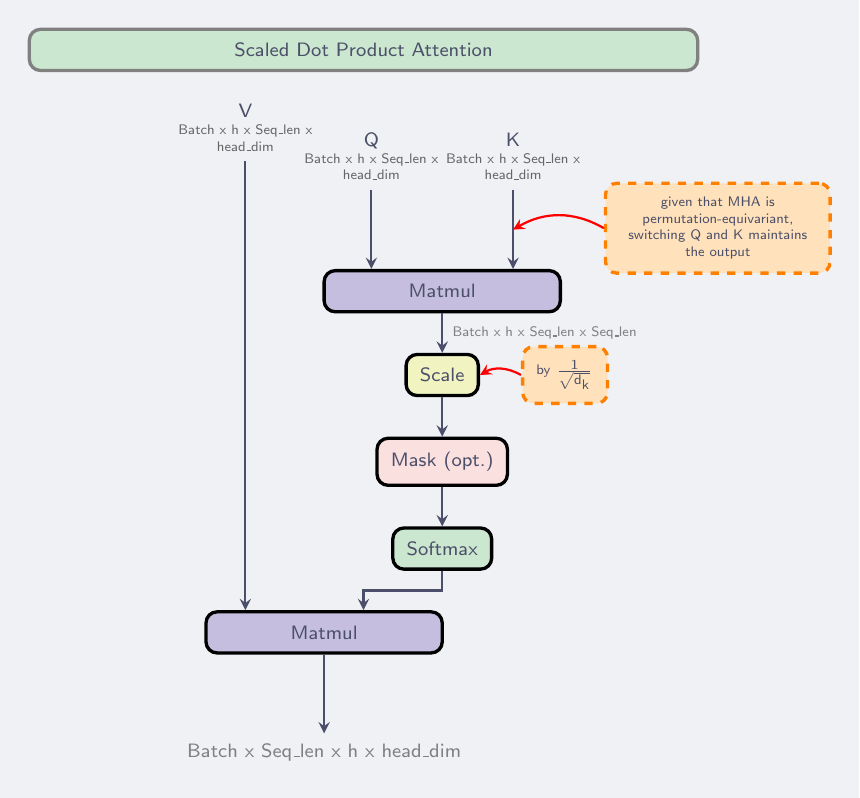
\begin{tikzpicture}[
          RIR/.style={draw=black, very thick, rectangle, rounded corners, inner sep=5pt, inner ysep=5pt}
          ]
          \tikzstyle{every node}=[font=\virgil\scriptsize]
          \node[RIR,fill=sgreen, draw=black!50, minimum width=0.7\textwidth] (sdpa) {Scaled Dot Product Attention};
          \node[RIR, anchor=north,minimum width=3cm,fill=spurple] (matmul) at ($(sdpa.south)+(1,-2.5)$) {Matmul};
          \node[RIR, anchor=north,fill=syellow] (scale) at ($(matmul.south)+(0,-0.5)$) {Scale};
          \node[RIR, anchor=north,fill=sstart] (mask) at ($(scale.south)+(0,-0.5)$) {Mask (opt.)};
          \node[RIR, anchor=north,fill=sgreen] (sm) at ($(mask.south)+(0,-0.5)$) {Softmax};
          \node[RIR, anchor=north,minimum width=3cm,fill=spurple] (matmul2) at ($(sm.south)+(-1.5,-0.5)$) {Matmul};
          % ARROWS
          \draw[<-,thick,>=stealth] ($(matmul.north)+(-0.9,0)$) -- ++ (0, 1) node[above]{\parbox{2cm}{\centering Q\\\tiny \textcolor{black!60}{Batch x h x Seq\_len x head\_dim}}};
          \draw[<-,thick,>=stealth] ($(matmul.north)+(0.9,0)$) -- ++ (0, 1) node[above]{\parbox{2cm}{\centering K\\\tiny \textcolor{black!60}{Batch x h x Seq\_len x head\_dim}}};
          \draw[->,thick,>=stealth] (matmul) -- node[right]{\tiny \textcolor{black!50}{Batch x h x Seq\_len x Seq\_len}} (scale);
          \draw[->,thick,>=stealth] (scale) -- (mask);
          \draw[->,thick,>=stealth] (mask) -- (sm);
          \draw[->,thick,>=stealth] (sm.south) |- ($(matmul2.north)+(0.5,0.25)$) -- ($(matmul2.north)+(0.5,0)$);
          \draw[<-,thick,>=stealth] ($(matmul2.north)+(-1,0)$) -- ++ (0,5.7) node[above]{\parbox{2cm}{\centering V\\\tiny \textcolor{black!60}{Batch x h x Seq\_len x head\_dim}}};
          \draw[->,thick,>=stealth] (matmul2.south) -- ++ (0,-1) node[below]{\textcolor{black!50}{Batch x Seq\_len x h x head\_dim}};
          % explaining 
        \node [RIR, fill=sorange, draw=orange,dashed] (lrich) at ($(matmul)+(3.5,0.8)$) {
            \parbox{2.5cm}{\tiny \centering given that MHA is permutation-equivariant, switching Q and K maintains the output}
            };
        \draw [->,thick,red,>=stealth] (lrich.west) to [out=150,in=30] ($(matmul.north)+(0.9,0.5)$);
        % comment on scale
        \node [RIR, fill=sorange, anchor=west, draw=orange,dashed] (lscale) at ($(scale)+(1,0)$) {
            \tiny \centering by $\frac{1}{\sqrt{\text{d\textsubscript{k}}}}$};
        \draw [->,thick,red,>=stealth] (lscale.west) to [out=150,in=30] (scale.east);
        \end{tikzpicture}
      \end{figure}
      From the diagram above, there's a new block, \bandi{Mask}, that does something called masking. A transformer usually has two phases,
      encoding phase and the decoding phase. From the Transformers architecture diagram, encoder is on the left and the decoder on the right 
      for the two phases.
\end{minipage}%
\hspace{25pt}
\begin{minipage}[t]{.4\textwidth}
  \raggedright
  \scriptsize 
    \fontsize{9}{8}\textcolor{xtitle}{\it from previous $^{13}$...}\\
    \begin{itemize}[left=0pt,topsep=0pt,itemsep=-1ex,parsep=0ex]
        \item \textbf{\textit{values}} {\tiny $\sim$} for each input element, we also have a value vector. This feature vector is the one we want to average over.
        \item \textbf{\textit{score function}} {\tiny $\sim$} to rate which elements we want to pay attention to, we need to specify a score function. The score function 
        takes the query and a key as input, and outputs the score (attention weight) of the query-key pair. It is usually implemented by simple similarity metrics like 
        a dot product, or a small MLP.
    \end{itemize}
    
\includegraphics[width=.1\textwidth]{images/hand-point-up.png}
    \textbf{
                \textit{courtesy of \href{https://uvadlc-notebooks.readthedocs.io/en/latest/tutorial_notebooks/tutorial6/Transformers_and_MHAttention.html}{UvA course notes}}
                }\\
    \vspace{2em}
    {\sidecitecount} $d_k$ is the size of the last dimension of the keys after linear projection and transpose, to be implemented later.
    It is the head dimension for each attention head.\\ 
    Sanity check states that your key dimension be {\it B x Seq\_len x h x head\_dim}
    before this step where $d_k$ is gotten by {\it k.shape[-1]}
\end{minipage}
\end{figure}
\pagebreak 
% PAGE 8
\begin{figure}[!htb]
    \begin{minipage}[t]{0.65\textwidth}
    \raggedright
    During the decoding phase, at each step of predicting a word{\maincitecount}, the network needs take a look 
    at the words previous to that step, and output a softmax prediction for what it thinks the next word 
    is. Since transformers attend to the entire sequence, before and after, it becomes a trivial task to predict 
    the next word, simply by putting 100\% attention to the word after it.\\
    This of course is cheating, it won't learn anything really. During the inference pipeline, the entire sequence 
    won't be present, hence why we need the masking block, we don't want each word in the decoder to see the words 
    that come after it.\\
    \customtext{xtitle}{1em}{Implementing masking in code}\\
    Let's use the sequence below\\
    {\it Eiffel Tower is in Paris}\\
    and consider the llama 2 tokenizer{\maincitecount}, {\it sentencepiece}, as the final Transformers model built on these progressive learnings  
    while building on the architecture is Llama 2.
\begin{lstlisting}[language=python,style=python,basicstyle=\ttfamily\footnotesize]
import sentencepiece as spm 
sequence = "Eiffel Tower is in Paris"
sp = spm.SentencePieceProcessor("llama-2-7b-tok.model")
tokens = sp.encode_as_ids(sequence)
\end{lstlisting}
Considering V and D used for {\it Llama2 model 7B} variant, let's initialize an embedding instance. 
\begin{lstlisting}[language=python,style=python,basicstyle=\ttfamily\footnotesize]
V,D=32_000,4_096
emb = nn.Embedding(V, D)
emb_tokens = emb(torch.tensor(tokens))
print(emb_tokens.shape)
# torch.Size([7, 4096])
\end{lstlisting}
Our embeddings output being the input to scaled dot product attention, let's compute $QK^T$ then scale
keeping in mind that the batch dimension, multiple heads, and the positional encoding is not incorporated 
for the sake of focusing on masking.
\begin{lstlisting}[language=python,style=python,basicstyle=\ttfamily\footnotesize]
Wq, Wk, Wv = nn.Linear(D,D),nn.Linear(D,D),nn.Linear(D,D)
q, k, v = Wq(emb_tokens), Wk(emb_tokens), Wv(emb_tokens)
scores=q@k.T
scaled_scores=scores/k.shape[-1]**.5
print(scaled_scores.shape) # torch.Size([7, 7])
\end{lstlisting}
% weights=torch.softmax(scaled_scores,dim=-1)
\end{minipage}%
\hspace{25pt}
\begin{minipage}[t]{.4\textwidth}
  \raggedright
  \scriptsize 
  {\sidecitecount} the model actually predicts a token which, by using a lookup table, is decoded to a word which 
  is what humans understand.\\
  \vspace{2em}
  {\sidecitecount} the lookup-table {\it tokenizer.model} can be found from the huggingface model card for {\it Llama-2-7b}
  {\scriptsize \url{https://huggingface.co/meta-llama/Llama-2-7b/tree/main}}
\end{minipage}
\end{figure}
\pagebreak
% PAGE 9
\begin{figure}[!htb]
    \begin{minipage}[t]{0.65\textwidth}
    \raggedright
    
\begin{lstlisting}[language=python,style=python,basicstyle=\ttfamily\tiny]
torch.set_printoptions(precision=5,sci_mode=False,linewidth=500)
print(scaled_scores)
tensor([[-0.10457, -0.23802,  0.08053,  0.33000, -0.10408,  0.55068,  0.68916],
        [-0.35013, -0.04846,  0.65688,  0.18756, -0.81784,  0.10682, -0.74313],
        [-0.26961, -0.70423,  0.94224,  0.16090, -0.20169,  0.15549, -0.28134],
        [-0.32253,  0.56740,  0.08793, -0.53429, -0.19362, -0.22245, -0.38808],
        [ 0.32020,  0.29380,  0.18501, -0.53281,  0.02592, -0.57664,  0.17737],
        [ 0.00706, -0.08485, -0.11895,  0.21021,  0.50643,  0.48187,  0.11625],
        [ 0.38275,  0.45847, -0.34459, -0.12443,  0.35930,  0.65530,  0.03805]], 
        grad_fn=<DivBackward0>)
\end{lstlisting}
Now onto a mask with ones from the first upper off-diagonal onwards. Then, fill them with {\small $-\infty$}
such that the exponential of those values will be zero in the weights. 
\begin{lstlisting}[language=python,style=python,basicstyle=\ttfamily\footnotesize]
mask = torch.triu(torch.ones_like(scaled_scores), diagonal=1)
scaled_scores_masked = scaled_scores.masked_fill_(mask.bool(), -torch.inf)
weights = torch.softmax(scaled_scores_masked, dim=-1)
\end{lstlisting}
Now, for the weights, pre-matrix multiply with {\small V} for the result of Scaled Dot Product Attention
\begin{lstlisting}[language=python,style=python,basicstyle=\ttfamily\footnotesize]
out = weights @ v 
print(out.shape) # torch.Size([7, 4096])
\end{lstlisting}
Nice! Now onto {\it Add \& Norm} layer, which from the paper, is a Layer normalization that computes\\
\vspace{-1.5em}
$$\text{LayerNorm}(x  + \text{Multihead(}x))$$
where $x$ is basically the same sequence (as an embedding) input to the $Q, K \& V$. This layer hence
is a residual connection necessary for enabling smooth gradient flow through the model and retaining 
information from the original sequence prior to the multi-head attention. This is simply implemented as 
\begin{lstlisting}[language=python,style=python,basicstyle=\ttfamily\footnotesize]
out_attn = multiheadAttn(x)
out = x + out_attn
norm_out = norm(out)
\end{lstlisting}
\customtext{xtitle}{0em}{What about the Feed Forward Network layer}\\
Always forming a crucial layer in most models, the FFN, in this case, 
maps context rich vectors onto a higher dimension{\maincitecount} which 
increases learning so it can model more complex relationships and also 
adds an activation function to introduce non-linear, even better relations.
\end{minipage}%
\hspace{25pt}
\begin{minipage}[t]{.4\textwidth}
  \raggedright
  \centering
  \scriptsize 
  {\sidecitecount} \textcolor{xtitle}{\it Feed Forward NN layer for Transformer model}\\
  \vspace{1em}
    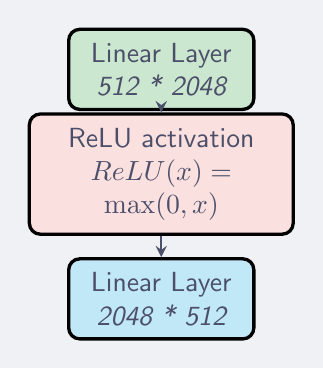
\begin{tikzpicture}[
    BIR/.style={rectangle, draw=black!60, fill=black!5, very thick, minimum size=5mm, minimum height=4em, minimum width=6em},
    RIR/.style={draw=black, very thick, rectangle, rounded corners, inner sep=5pt, inner ysep=5pt}
    ]
        \node[RIR, fill=sgreen] (L1) {\parbox{2cm}{\centering Linear Layer\\{\it 512 * 2048}}};
        \node[RIR, fill=sstart] (L2) at  ($(L1.south)+(0,-0.8)$) {\parbox{3cm}{\centering ReLU activation\\{$ReLU(x)=\max(0,x)$}}};
        \draw[thick,->,>=stealth] (L1.south) -- (L2.north);
        \node[RIR, fill=sblue] (L3) at  ($(L2.south)+(0,-0.8)$) {\parbox{2cm}{\centering Linear Layer\\{\it 2048 * 512}}};
        \draw[thick,->,>=stealth] (L2.south) -- (L3.north);
    \end{tikzpicture}\\
  \vspace{1em}
  \textcolor{xtitle}{\it Feed Forward NN layer for GPT-2}\\
  \vspace{0.5em}
    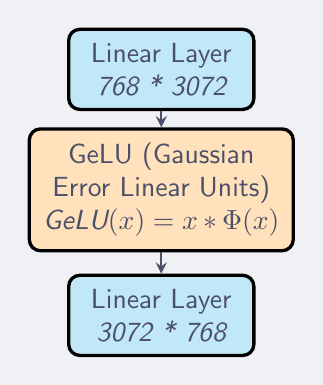
\begin{tikzpicture}[
    BIR/.style={rectangle, draw=black!60, fill=black!5, very thick, minimum size=5mm, minimum height=4em, minimum width=6em},
    RIR/.style={draw=black, very thick, rectangle, rounded corners, inner sep=5pt, inner ysep=5pt}
    ]
        \node[RIR, fill=sblue] (L1) {\parbox{2cm}{\centering Linear Layer\\{\it 768 * 3072}}};
        \node[RIR, fill=sorange] (L2) at  ($(L1.south)+(0,-1)$) {\parbox{3cm}{\centering GeLU (Gaussian Error Linear Units)\\{$\text{\it GeLU}(x)=x*\Phi(x)$}}};
        \draw[thick,->,>=stealth] (L1.south) -- (L2.north);
        \node[RIR, fill=sblue] (L3) at  ($(L2.south)+(0,-0.8)$) {\parbox{2cm}{\centering Linear Layer\\{\it 3072 * 768}}};
        \draw[thick,->,>=stealth] (L2.south) -- (L3.north);
    \end{tikzpicture}
    \vspace{1em}\\
    \textcolor{xtitle}{\it Feed Forward NN layer for Llama-2-7b}\\
    \vspace{0.5em}
    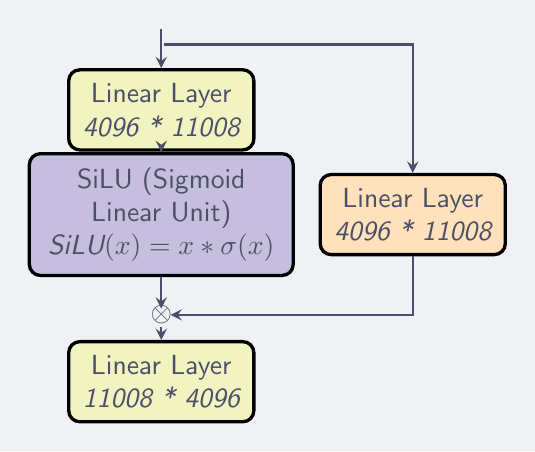
\begin{tikzpicture}[
    BIR/.style={rectangle, draw=black!60, fill=black!5, very thick, minimum size=5mm, minimum height=4em, minimum width=6em},
    RIR/.style={draw=black, very thick, rectangle, rounded corners, inner sep=5pt, inner ysep=5pt}
    ]
        \node[RIR, fill=syellow] (L1) {\parbox{2cm}{\centering Linear Layer\\{\it 4096 * 11008}}};
        \draw[>=stealth,thick,<-] (L1.north) -- ++ (0,0.5) node[pos=0.6,name=l1c,inner sep=0]{};
        \node[RIR, fill=spurple] (L2) at  ($(L1.south)+(0,-0.8)$) {\parbox{3cm}{\centering SiLU (Sigmoid Linear Unit)\\{$\text{\it SiLU}(x)=x*\sigma(x)$}}};
        \node[RIR, fill=sorange, anchor=west] (LV) at ($(L2.east)+(0.3,0)$) {\parbox{2cm}{\centering Linear Layer\\{\it 4096 * 11008}}};
        \draw[>=stealth,thick,->] (l1c) -| (LV.north);
        \draw[thick,->,>=stealth] (L1.south) -- (L2.north);
        \draw[thick,->,>=stealth] (L2.south) -- ++ (0,-0.4) node[name=hp,pos=1.2]{$\otimes$};
        \draw[thick,->,>=stealth] (LV.south) |- ($(hp.east)+(-0.15,0)$);
        \node[RIR, fill=syellow] (L3) at  ($(hp.south)+(0,-0.6)$) {\parbox{2cm}{\centering Linear Layer\\{\it 11008 * 4096}}};
        \draw[thick,->,>=stealth] ($(hp.south)+(0,0.1)$) -- (L3.north);
    \end{tikzpicture}
\end{minipage}
\end{figure}
\pagebreak
% PAGE 10
\begin{figure}[!htb]
    \begin{minipage}[t]{0.65\textwidth}
    \raggedright
    \customtext{xtitle}{0em}{Building Llama-2 from the SDPA outwards...}\\
Gladly having gone through the layers in the Transformer model, it is of essence 
to build the Llama-2 model graph and load the weights for the 7B variant. 
It is a decoder-only architecture, as is most State of The Art common LLMs.
Why is that?\\
Well, decoder-only architectures worked very well for next token prediction and translation tasks, 
and were easier to train. And so, they picked up as the {\it de facto} baselines for most current
outstanding models.\\
Earlier, we had the graph for the Multi-head Attention, let's add codes to it to map it 
to implementation.\\
\begin{tikzpicture}[
    BIR/.style={rectangle, draw=black!60, fill=black!5, very thick, minimum size=5mm, minimum height=4em, minimum width=6em},
    RIR/.style={draw=black,thick,rectangle,rounded corners,inner sep=5pt, inner ysep=5pt}
    ]
    \tikzstyle{every node}=[font=\virgil\scriptsize]
    \node (ref) at (0,0){}; % needs be set as global coordinate
    % node for embeddings
    \node[RIR,fill=sstart] (head) at ($(ref.east)+(-10, -1.1)$) {\parbox{4cm}{
        \centering embeddings\\{
            \usebox{\codebox}
            }}};
    % explaining embeddings
    \node [RIR, fill=sorange, draw=orange,dashed] (lrich) at ($(head)+(4, 0)$) {\parbox{2.5cm}{\tiny \centering high-dimensional latent rich token representation as input}};
    \draw [->,thick,red,>=stealth] (lrich.west) to [out=150,in=30] (head.east);
    % three arrows extengin from ebeddings
    \draw[->, thick,>=stealth] (head.south) -- node[name=midh,inner sep=0, outer sep=0]{} node[pos=0.25,right]{{\tiny embeddings denoted as x}} ++ (0, -0.8) node[name=endl1, inner sep=0]{};
    \draw[->, thick,>=stealth] (midh) -- ++ (5,0) -- ++ (0, -0.3) node[name=endl2, inner sep=0]{};
    \draw[->, thick,>=stealth] (midh) -- ++ (-5,0) -- ++ (0, -0.3) node[name=endl3, inner sep=0]{};
    % nodes for matrix multiplication
    \node[RIR,fill=sblue, anchor=north] (q) at (endl3) {
        \parbox{3.8cm}{\centering Q=W\textsubscript{q}(x)\\
        \usebox{\codeq}
        }};
    \node[RIR,fill=sblue, anchor=north] (k) at (endl1) {
        \parbox{3.8cm}{
            \centering K=W\textsubscript{k}(x)
            \usebox{\codek}
        }};
    \node[RIR,fill=sblue, anchor=north] (v) at (endl2) {
        \parbox{3.8cm}{\centering
        V=W\textsubscript{v}(x)\\
        \usebox{\codev}
    }};
    % explain expand nodes
    \node [RIR, draw=black,dashed,fill=sblue, anchor=west] at ($(v.east)+(0.5,0)$) {
        \parbox{2.5cm}{\tiny \centering W\textsubscript{q}, W\textsubscript{k}, and W\textsubscript{v} 
        are nn.Linear instances of dimensions \\(d\_out,d\_in)
        }
    };
    % arrows from Q to Qproj
    \draw[->, thick, >=stealth] (q.south) -- node[left]{\textcolor{black!50}{\parbox{2cm}{\tiny Batch x Seq\_len x d\_out}}} ++ (0,-0.7) node[name=q1]{};
    
    % nodes for projections of the q, k, and v h times
    \node[RIR, fill=syellow, anchor=north] (qproj) at (q1) {
    \parbox{3.5cm}{\tiny \centering linearly project Q h times\\\usebox{\projectq}}};
    \draw let \p1 = (qproj.north), \p2 = (k.south) in node[RIR, fill=syellow, anchor=north] (kproj) at (\x2, \y1) {
        \parbox{3.5cm}{\tiny \centering linearly project K h times\\\usebox{\projectk}}
    };
    \draw let \p1 = (qproj.north), \p2 = (v.south) in node[RIR, fill=syellow, anchor=north] (vproj) at (\x2, \y1) {
        \parbox{3.5cm}{\tiny \centering linearly project V h times\\\usebox{\projectv}}
    };
    % arrows from K, V to K proj, V proj respectively
    \draw[->, thick, >=stealth] (k.south) -- node[left]{\textcolor{black!50}{\tiny \parbox{1.8cm}{Batch x Seq\_len\\ x d\_out}}} (kproj.north) node[name=k1]{};
    \draw[->, thick, >=stealth] (v.south) -- node[left]{\textcolor{black!50}{\tiny Batch x Seq\_len x d\_out}} (vproj.north) node[name=v1]{};
    % explain expand nodes
    \node [RIR, draw=black,dashed,fill=syellow, anchor=west] at ($(vproj.east)+(0.2,-0.2)$) {
        \parbox{3cm}{\tiny \centering h=8 for the original Transformers architecture\\
        d\_out \% h == 0 must be met\\
        head\_dim = d\_out // h}
    };
    % SDPA node
    \node[RIR,fill=sgreen, draw=OliveGreen] (sdpa) at ($(kproj.south)+(0, -1.8)$) {Scaled Dot Product Attention};
    % arrows from projection nodes to SDPA
    \draw[->,thick,>=stealth] (qproj.south) |- node[left]{\textcolor{black!50}{
        \parbox{2cm}{\centering \tiny Batch x Seq\_len\\ x h x head\_dim}
        }
    } ($(sdpa.north)+(-1,0.3)$) -- ($(sdpa.north)+(-1,0)$);
    \draw[->,thick,>=stealth] (kproj.south) |- node[pos=0.3,left]{\textcolor{black!50}{
        \parbox{3cm}{\centering \tiny Batch x Seq\_len x h x head\_dim}
        }
    } ($(sdpa.north)+(0,0.3)$) -- (sdpa.north);
    \draw[->,thick,>=stealth] (vproj.south) |- node[pos=0.3,left]{\textcolor{black!50}{
        \tiny Batch x Seq\_len x h x head\_dim}
    } ($(sdpa.north)+(1,0.3)$) -- ($(sdpa.north)+(1,0)$);
    % output from SDPA node
    \node [RIR,anchor=north, fill=spurple] (outheads) at ($(sdpa.south)+(0,-0.8)$){
        \parbox{3.5cm}{
            \centering concatenate the heads\\
            \usebox{\concatheads}}};
    % arrow from SDPA to heads node
    \draw[->,thick,>=stealth] (sdpa.south) -- node[left,pos=0.5]{
        \parbox{3.5cm}{\tiny \centering output heads\quad head\textsubscript{1},...,head\textsubscript{h}\\
        \textcolor{black!50}{Batch x Seq\_len x h x head\_dim}
    }} (outheads.north);
    % Linear matrix multiplication 
    \node[RIR,fill=sblue,anchor=north] (lmm) at ($(outheads.south)+(0,-0.5)$) {
        \parbox{4cm}{\centering
      out = W\textsubscript{o}(concat\_h)\\
      \usebox{\projectout}
    }};
    % arrow from concat to linear mm
    \draw[->,thick, >=stealth](outheads.south) -- node[pos=0.5,left]{\textcolor{black!50}{\tiny Batch x Seq\_len x d\_out}} (lmm.north);
\end{tikzpicture}
% \begin{lstlisting}[language=python,style=python,basicstyle=\ttfamily\footnotesize]
% \end{lstlisting}
But wait! what about the RoPE implementation, remember that as has been discussed earlier,
positional encodings should be somewhere in the above disjointed{\maincitecount} graph of a code.
Let's figure out where?
\end{minipage}%
\hspace{25pt}
\begin{minipage}[t]{.4\textwidth}
  \raggedright
  \scriptsize 
  {\sidecitecount} disjointed for it does not exist in a {nn.Module} class with the updatable weights in the init
  part of the class  
\end{minipage}
\end{figure}
% ==================================================
\pagebreak
% PAGE 11
\begin{figure}[!htb]
    \begin{minipage}[t]{0.65\textwidth}
    \raggedright
    \customtext{xtitle}{0em}{Recap on Rotational Positional Encoding}\\
    \begin{tikzpicture}
        \node (intro) {
\begin{lstlisting}[language=python,style=python]
def precompute_freqs_cis(d, context_len, theta = 10_000, device = "gpu"):
    #
    #
    assert d % 2 == 0, "dim must be divisible by 2"
    #
    i_s = torch.arange(0,d,2)[:(d//2)].float()
    theta_s = theta ** (- i_s / d).to(device)
    m = torch.arange(context_len, device=device)
    freqs = torch.outer(m, theta_s).float()
    freqs_cis = torch.polar(torch.ones_like(freqs), freqs)
    return freqs_cis
\end{lstlisting}
        };
        \node (fAE) at ($(intro.north)+(2.9,-2.7)$){};
        % first arrow for the assertion
        \draw [->,red,>=stealth] ($(intro.north)+(4.5,-1.8)$) 
        node[name=fAS,right]{\parbox{3cm}{\centering \itred{As the paper\textsuperscript{\sidecite{9}} says, \enquote{\ldots to any $x_i\in R^d$ where d is even\ldots}}}} to 
        [out=180,in=10] (fAE.south);
        % second arrow for the i_s
        \draw [->,red,>=stealth] ($(intro.north)+(3.3,-4.5)$) 
        node[name=sabN]{} to 
        [out=180,in=-5] ($(intro.north)+(1.9,-4.05)$);
        \node[anchor=west] at (sabN) {\itred{
             \parbox{3cm}{\raggedright 
             $i_s=2(i-1)$ for $i\in\{1,2,\ldots,d/2\}$ 
             }}
        };
        % third arrow for the theta_s
        \draw [->,red,>=stealth] ($(intro.north)+(3.5,-5.5)$) to 
        [out=180,in=-5] ($(intro.north)+(1.7,-4.65)$);
        \node[anchor=west] at ($(intro.north)+(3.5,-5.5)$) {\itred{
             \parbox{6cm}{\raggedright 
             $10000^{-i_s/d}$ which expands to $10000^{-2(i-1)/d}$
             }}
        };
        % fourth arrow for the outer product
        \draw [->,red,>=stealth] ($(intro.north)+(3.5,-7.5)$) to 
        [out=180,in=-5] ($(intro.north)+(1.4,-5.75)$);
        \node[anchor=west] at ($(intro.north)+(3.5,-7.5)$) {\itred{
             \parbox{6cm}{\raggedright 
             outer product of $\vec{m}$ \& $\vec{\theta}$ to give
             \vspace{-2.5em}\\
             \tiny
             \[
             \begin{pmatrix}
                m_1\theta_1,\quad m_1\theta_2,\quad \ldots,\quad m_1\theta_{d/2-1},\quad m_1\theta_{d/2}\\
                m_2\theta_1,\quad m_2\theta_2,\quad \ldots,\quad m_2\theta_{d/2-1},\quad m_2\theta_{d/2}\\
                \mathbf{\vdots}\hspace{3.5em} \qquad \vdots\hspace{3.5em}\ldots\hspace{3.5em}\vdots\hspace{3.5em}\vdots\\
                m_{\text{cl}}\theta_1, m_{\text{cl}-1}\theta_2,\ldots, m_{\text{cl}-1}\theta_{d/2-1}, m_{\text{cl}-1}\theta_{d/2}\\
              \end{pmatrix}
              \]
             }}
        };
         % fifth arrow for the polar computation
         \draw [->,red,>=stealth] ($(intro.north west)+(5.8,-8.5)$) to 
         [out=180,in=-5] ($(intro.north west)+(2.8,-6.9)$);
         \node[anchor=west] at ($(intro.north west)+(5.8,-8.5)$) {\itred{
              \parbox{6cm}{\raggedright 
              elementwise mapping i.e.\\
              \tiny
              $m_1\theta_1 \Rightarrow \cos(m_1\theta_1)+i\sin(m_1\theta_1)$\\
              \scriptsize
              where the ones are the absolute value arguments
              }}
         };
\end{tikzpicture}
% \begin{tikzpicture}
% \node (intro) {
% \begin{lstlisting}[language=python,style=python,basicstyle=\ttfamily\footnotesize]
% def reshape_for_broadcast(freqs_cis: torch.Tensor, x: torch.Tensor):
%     ndim = x.ndim
%     assert 0 <= 1 < ndim
%     assert freqs_cis.shape == (x.shape[1], x.shape[-1])
%     shape = [d if i == 1 or i == ndim - 1 else 1 for i, d in enumerate(x.shape)]
%     return freqs_cis.view(*shape)
% \end{lstlisting}
% };
% \end{tikzpicture}
\begin{tikzpicture}
    \node (intro) {
\begin{lstlisting}[language=python,style=python,basicstyle=\ttfamily\footnotesize]
def apply_rotary_embs(x, freqs_cis, device):
    #
    #
    x_c = torch.view_as_complex(
        x.float().reshape(*x.shape[:-1], -1, 2)
    ) 
    #
    f_c = freqs_cis.unsqueeze(0).unsqueeze(2)
    #
    #
    x_rotated = x_c * f_c
    #
    x_out = torch.view_as_real(x_rotated)
    #
    x_out = x_out.reshape(*x.shape)
    return x_out.type_as(x).to(device)
\end{lstlisting}
    };
    % first arrow to expand dims
    \draw [->,red,>=stealth] ($(intro.north east)+(1.5,-2.6)$) to 
    ($(intro.north east)+(0,-2.6)$);
    \node[anchor=west] at ($(intro.north east)+(1.5,-2.6)$) {\itred{
            \parbox{6cm}{\raggedright 
            dynamically expands the last dimension \\
            (\ldots,d1) to \big(\ldots,$\frac{d1}{2}$,2\big) where d1 is even
            }}
    };
    % second arrow to convert to complex
    \draw [->,red,>=stealth] ($(intro.north east)+(2.5,-0.4)$) 
    node[name=send]{} to 
    [out=180,in=0] ($(intro.north)+(1.5,-2.1)$);
    \node[anchor=west] at (send) {\itred{
            \parbox{6cm}{\raggedright
            takes each group of 2s of elements,\dots\newline
            [x, y],\newline
            [m, n],
            \ldots\\
            to single elements of\\
            x+yj,\\m+jn\ldots
            }}
    };
    % third arrow 
    \draw [->,red,>=stealth] ($(intro.north west)+(3.5,-3.5)$) node[name=se]{} to 
    [out=180,in=-5] ($(intro.north west)+(1.4,-2.1)$);
    \node[anchor=west] at (se) {\itred{
            \parbox{6cm}{\raggedright 
            dims transformed from $\left(\ldots,d\right)$\quad to\quad $\left(\ldots,\frac{d}{2}\right)$
            }}
    };
    % fourth arrow
    \draw [->,red,>=stealth] ($(intro.south)+(5.5,1)$) node[name=se]{} to 
    [out=180,in=-5] ($(intro.south)+(3.1,2.05)$);
    \node[anchor=west] at (se) {\itred{
            \parbox{6cm}{\raggedright 
            reverses the effect of torch.view\_as\_complex
            }}
    };
\end{tikzpicture}
With the knowledge of the implementation of the rotational positional encodings, 
let's inject it into the graph for the MultiHead Attention after the transformation 
\vspace{-1em}
\begin{gather*}
    [\text{\it batch} \times \text{\it seq\_len} \times \text{\it n\_heads} \times \text{\it head\_dim}]
\end{gather*}
\vspace{-3em}\\
but before the high-dimensional transpose to get the batch of heads each with dimensions (seq\_len,head\_dim){\maincitecount}.
% \begin{lstlisting}[language=python,style=python,basicstyle=\ttfamily\footnotesize]
% \end{lstlisting}
\end{minipage}%
\hspace{25pt}
\begin{minipage}[t]{.4\textwidth}
  \raggedright
  \scriptsize 
  {\sidecitecount} reminder that the rotational transformation is to be applied to the queries and keys only and not the values
  ({\it refer to page 4}).
\end{minipage}
\end{figure}
% ==================================================
\pagebreak
% PAGE 12
\begin{figure}[!htb]
    \begin{minipage}[t]{0.65\textwidth}
    \raggedright
$\star$ which is then done below{\maincitecount}\\
\begin{tikzpicture}
\node (intro) {
\begin{lstlisting}[language=python,style=python,basicstyle=\ttfamily\footnotesize]
# Already defined earlier 
dim=4096; n_heads=32; context_len=4096
Q,K,V=... # each dims being (Batch,SeqLen,Heads,HDim)
m_theta_polar_tensor = precompute_freqs_cis(dim//n_heads, context_len*2,"cpu")
m_theta_polar_seq = m_theta_polar_tensor[:seq_len]
Q=apply_rotary_emb(Q,m_theta_polar_seq)
K=apply_rotary_emb(K,m_theta_polar_seq)
\end{lstlisting}
};
\end{tikzpicture}
\customtext{xtitle}{0em}{Unwrapping the Transformer Block}\\
As much as the original Transformer does the normalization as
\vspace{-1em}
$$\text{LayerNorm}(x  + \text{Multihead(}x))$$
\vspace{-2.7em}\\
Llama2 does a prenormalization given by
\vspace{-1em}
\begin{align*}
    x_n & = \text{RMSNorm}(x)\\
    \text{out} & = x  + \text{Multihead(}x_n)\\
    & \text{\small where}\\
    & \text{\small RMSNorm($x$)}=\frac{x_i}{\text{\small RMS}(x)}*\gamma_i\\
    & \text{\small RMS($x$)} = \sqrt{\epsilon+\frac{1}{n}\sum_{i=1}^nx_i^2}
\end{align*}
\vspace{-1.5em}\\
which works out in code as 
\begin{lstlisting}[language=python,style=python,basicstyle=\ttfamily\footnotesize]
class RMSNorm(torch.nn.Module):
    def __init__(self, dim: int, eps: float = 1e-5):
        super().__init__()
        self.eps = eps
        self.weight = nn.Parameter(torch.ones(dim))
    def forward(self, x):
        means = x.pow(2).mean(-1, keepdim=True)
        norm_x = x * torch.rsqrt(means + self.eps)
        return (norm_x * self.weight).to(x.dtype)

rmsNorm=RMSNorm(dim) # dim=4096
x_norm=rmsNorm(x) # x => embeddings => (Batch,SeqLen,Dim)
# some mhAttention already instantiated called below 
attn_out=mhAttention(x_norm)
# then add 
out = x + attn_out
\end{lstlisting}
with the pre-normalization done to the input to the attention block and 
to the input to the  feed-forward networks. 
% \begin{lstlisting}[language=python,style=python,basicstyle=\ttfamily\footnotesize]
% \end{lstlisting}
\end{minipage}%
\hspace{25pt}
\begin{minipage}[t]{.4\textwidth}
  \raggedright
  \scriptsize 
  {\sidecitecount} full neat implementation\\
  \url{https://github.com/Marvin-desmond/ScalingViTsAcrossTrainingCompute/blob/main/mha/mha_with_rope.py}\\
  {\it Llama 2 Multi-Head Attention with ROPE}
\end{minipage}
\end{figure}
% ==================================================
\pagebreak
% PAGE 13
\begin{figure}[!htb]
    \begin{minipage}[t]{0.65\textwidth}
    \raggedright
    However, the original FFN, as can be seen from the side notes 
    on {\it pg.9}, does two linear transformations with a 
    ReLU{\maincitecount} activation function applied between the two 
    linear transformations.
    \begin{align*}
        FFN(x, W_1, W_2, b_1, b_2) = \max(0, xW_1 + b_1)W_2 + b_2
    \end{align*}
    the above equation being representative of the graph computation in the 
    linear topology on the just aforementioned page.\\
    Llama2, the current LLM architecture of interest in implementation in this 
    section of the article, 
    focuses on a Linear Unit known as SwiGLU{\maincitecount}, 
    a variation of the Transformer FFN layer which then uses a variant of the 
    Gated Linear Unit{\maincitecount}.
    This leads to the FFN layer having three weight matrices as opposed to the original two 
    which yields the implementation below.
    \begin{tikzpicture}[
    BIR/.style={rectangle, draw=black!60, fill=black!5, very thick, minimum size=5mm, minimum height=4em, minimum width=6em},
    RIR/.style={draw=black, very thick, rectangle, rounded corners, inner sep=3pt, inner ysep=5pt}
    ]
        \footnotesize
        \node[] (ref) {};
        \node[RIR, fill=syellow] (L1) at ($(ref.south)+(0,-2)$) {\parbox{2cm}{\centering Linear Layer\\{\it (4096,11008)}}};
        \draw[>=stealth,thick,<-] (L1.north) -- ++ (0,0.5) node[pos=0.6,name=l1c,inner sep=0]{};
        \node[RIR, fill=spurple,anchor=north] (L2) at  ($(L1.south)+(0,-0.8)$) {\parbox{3cm}{\centering Sigmoid Linear Unit\\{$\text{\it SiLU}(x)=x*\sigma(x)$}}};
        \node[RIR, fill=sorange, anchor=west] (LV) at ($(L2.east)+(0.3,0)$) {\parbox{2cm}{\centering Linear Layer\\{\it (4096,11008)}}};
        \draw[>=stealth,thick,->] (l1c) -| (LV.north);
        \draw[thick,->,>=stealth] (L1.south) -- (L2.north);
        \draw[thick,->,>=stealth] (L2.south) -- ++ (0,-0.4) node[name=hp,pos=1.2]{$\otimes$};
        \draw[thick,->,>=stealth] (LV.south) |- ($(hp.east)+(-0.15,0)$);
        \node[RIR, fill=syellow] (L3) at  ($(hp.south)+(0,-1)$) {\parbox{2cm}{\centering Linear Layer\\{\it (11008,4096)}}};
        \draw[thick,->,>=stealth] ($(hp.south)+(0,0.1)$) -- (L3.north);
        % IMAGE POINTING TO THE CODE
        \node[anchor=west] (hand) at ($(LV.east)+(0.1,0)$) {\includegraphics[width=0.15\textwidth]{images/hand-point-right.png}};
        % THE CODE FOR LLAMA 2 FFN
            \node[RIR,fill=sblue,anchor=west] (lmm) at ($(hand.east)+(0.1,0)$) {
            \parbox{10cm}{\centering
            \usebox{\ffnllama}
            }};
    \end{tikzpicture}
    With the $\star$ operation being the Hadamard product, or as commonly known, 
    the elementwise product, of the two Weight matrices of dimensions 
    {\it $(4096,11008)$} to give a resulting matrix maintaining the given dimensions.\\
    In the general implementation for any given Llama 2 variant, the hidden dimension size is 
    gotten by 
    \begin{itemize}[left=0pt,topsep=0pt,itemsep=0ex,parsep=0ex]
        \item scaling of {\it dim} by 4
        \item reduction by $2/3$
        \item adjust it as a factor of a given multiple for computational efficiency
      \end{itemize}
\end{minipage}%
\hspace{25pt}
\begin{minipage}[t]{.4\textwidth}
  \raggedright \scriptsize
  {\sidecitecount} \href{https://proceedings.mlr.press/v15/glorot11a.html}{https://proceedings.mlr.press/v15/glorot11a.html}\\
  {\it Deep Sparse Rectifier Neural Networks}\\
  {\it Glorot et al. 2011}\\
  \vspace{2em}
  {\sidecitecount} \href{https://arxiv.org/abs/2002.05202v1}{https://arxiv.org/abs/2002.05202v1}\\
  {\it GLU Variants Improve Transformer}\\
  {\it Noam Shazeer 2020}\\
  \vspace{2em}
  {\sidecitecount} \href{https://arxiv.org/abs/1606.08415}{https://arxiv.org/abs/1606.08415}\\
  {\it Gaussian Error Linear Units (GELUs)}\\
  {\it Dan Hendrycks, Kevin Gimpel 2016}
\end{minipage}
\end{figure}
% ==================================================
% ==================================================
\pagebreak
% PAGE 14
\begin{figure}[!htb]
    \begin{minipage}[t]{0.95\textwidth}
        \raggedright
        Hence, from the clarifications, the whole Transformer block is visualized as
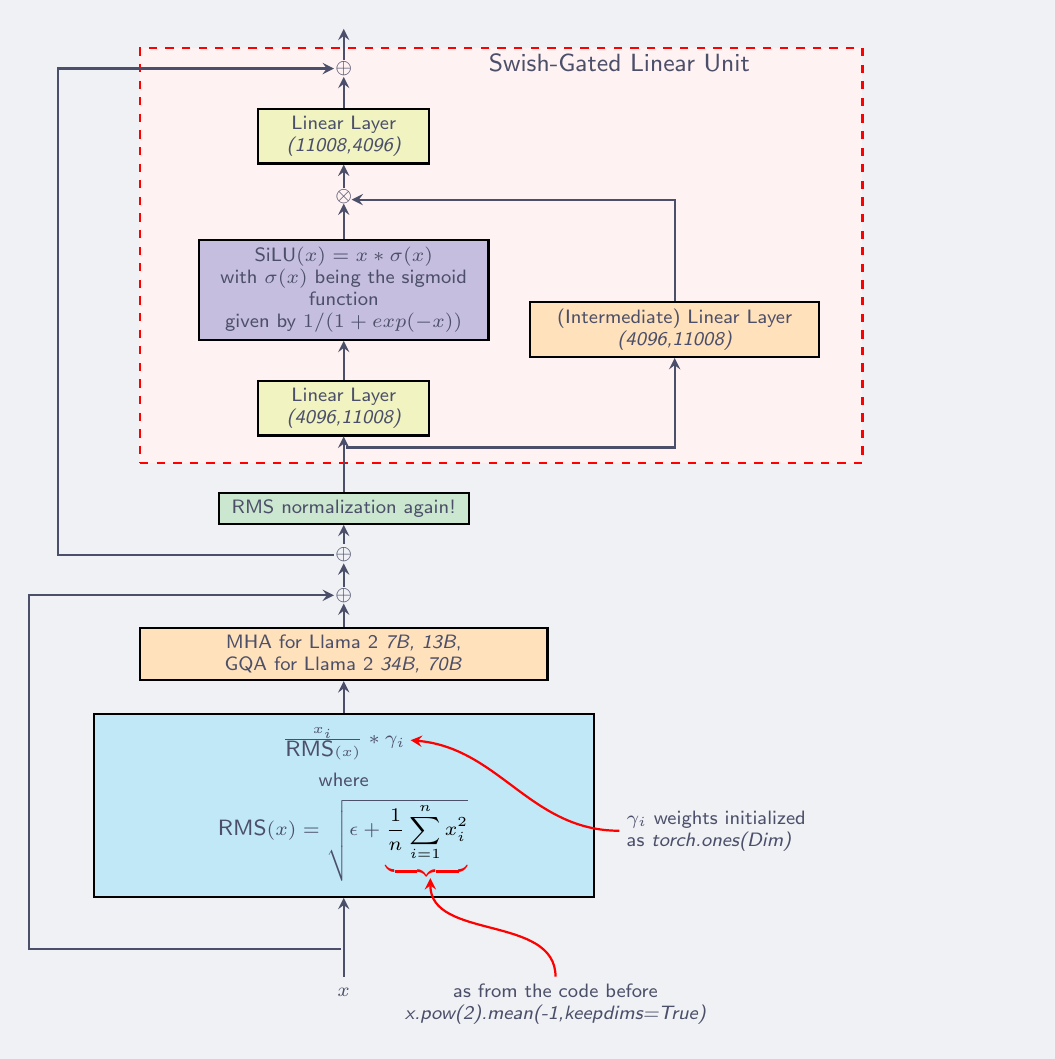
\begin{tikzpicture}[RIR/.style={draw=black,thick,rectangle},AR/.style={->,thick,>=stealth}]
    \scriptsize 
    % RMS Pre-Normalization
    \node[RIR,fill=sblue,inner sep=5pt] (prenorm) {\parbox{6cm}{\centering $\frac{x_i}{\text{\footnotesize RMS}(x)}*\gamma_i$\vspace{0.5em}\\where\vspace{0.5em}\\$\text{\footnotesize RMS}(x)=\sqrt{\epsilon+{\color{red} \underbrace{\color{black} \frac{1}{n}\sum_{i=1}^nx_i^2}}}_{}$}};
    % MHA Block (Abstracted as already iimplemented)
    \node[RIR,fill=sorange,anchor=south] (mha) at ($(prenorm.north)+(0,0.4)$) {\parbox{5cm}{\centering MHA for Llama 2 \textit{7B, 13B}, \\GQA for Llama 2 \textit{34B, 70B}}};
    % Add the Attention Output and the original Input
    \draw[<-,thick,>=stealth] (prenorm.south) -- node[name=fromx,pos=0.65,inner sep=0pt]{} ++ (0,-1) node[pos=1.2]{$x$};
    % Implement the RMS Again
    \node[RIR,anchor=south,fill=sgreen] (prermsffn) at ($(mha.north)+(0,1.3)$) {
        \parbox{3cm}{\centering RMS normalization again!}
        };
    % WRAPPING BOX FOR SWIGLU
    \node[RIR,anchor=south,fill=red!5,draw=red,dashed,minimum height=5.2cm,minimum width=9cm] at ($(prermsffn.north)+(2,0.35)$) {
        \parbox[t][5.1cm][t]{9cm}{
        \centering\virgil \fontsize{9}{10}\selectfont \hspace{3cm}Swish-Gated Linear Unit}
        };
    % FFN after the normalization
    \node[RIR, fill=syellow,anchor=south] (L1) at ($(prermsffn.north)+(0,0.7)$) {\parbox{2cm}{\centering Linear Layer\\{\it (4096,11008)}}};
        \node[RIR,fill=spurple,anchor=south] (L2) at  ($(L1.north)+(0,0.5)$) {\parbox{3.5cm}{\centering 
        SiLU$(x)=x*\sigma(x)$\\
        {with $\sigma(x)$ being the sigmoid function}\\
        {given by} $1/(1+exp(-x))$
        }};
        \draw[thick,->,>=stealth] (L1.north) -- (L2.south);
        \draw[thick,->,>=stealth] (L2.north) -- ++ (0,0.45) node[pos=1.2,name=ct,inner sep=0]{$\mathbf{\otimes}$};
        \draw[AR] (ct.north) -- ++ (0,0.3) node[name=ctend]{};
        \node[RIR, fill=syellow,anchor=south] (L3) at  (ctend) {\parbox{2cm}{\centering Linear Layer\\{\it (11008,4096)}}};
    % ir linear layer
    \node[RIR,anchor=west,fill=sorange] (irlayer) at ($(L2.east)+(0.5,-0.5)$) {\parbox{3.5cm}{
    \centering \scriptsize (Intermediate) Linear Layer\\
    \it (4096,11008)
    }};
    % ARRROWS 
    % PreNorm to MHA
    \draw[AR] (prenorm.north) -- (mha.south);
    % MHA to FFN VIA RMS NORM AGAIN
    \draw[AR] (mha.north) -- ++ (0,0.3) node[name=conc1,anchor=south,inner sep=0]{\scriptsize $\oplus$};
    \draw[AR] (conc1.north) -- ++ (0,0.3) node[name=conc2,anchor=south,inner sep=0]{\scriptsize $\oplus$};
    \draw[AR,<-] (prermsffn.south) -- ++ (0,-0.25);
    \draw[->,thick,>=stealth] (fromx) -- ++ (-4,0) |- (conc1.west);
    \draw[AR] (prermsffn.north) -- node[pos=0.8,inner sep=0pt,name=midtoir]{} (L1.south);
    % INPUT TO L1 TAPPED TO IR LINEAR LAYER
    \draw[AR] (midtoir) -| (irlayer.south);
    \draw[AR] (irlayer.north) |- ($(L2.north)+(0.1,0.5)$);
    % L3 TO OUT
    \draw[AR] (L3.north) -- ++ (0,0.4) node[name=conc3,anchor=south,inner sep=0]{\scriptsize $\oplus$};
    \draw[AR] (conc3.north) -- ++ (0,0.4);
    % RMS AGAIN TO OUT
    \draw[AR] (conc2.west) --++ (-3.5,0) |- (conc3.west);
    % Explain code
    \draw [->,red,thick,>=stealth] ($(prenorm.north)+(3.5,-1.5)$) node[name=pnw]{} to 
    [out=180,in=-5] ($(prenorm.north)+(0.85,-0.35)$);
    \node[anchor=west] at (pnw) {
            \parbox{5cm}{\raggedright \virgil
            $\gamma_i$ weights initialized\\ as \normalfont \it torch.ones(Dim)
            }
    };
    % explain underbrace
        \draw [->,red,thick,>=stealth] ($(prenorm.south east)+(-0.5,-1)$) node[name=uc]{} to [out=90,in=-90] ($(prenorm.south)+(1.1,0.25)$);
    \node[anchor=north] at (uc) {
            \parbox{6cm}{\centering \virgil
            as from the code before\\
            {\normalfont \textit{x.pow(2).mean(-1,keepdims=True)}}
            }
    };
\end{tikzpicture}\\
With the above nice input-output mapping translating to code as
\begin{lstlisting}[language=python,style=python,basicstyle=\ttfamily\footnotesize]
class TransformerBlock(nn.Module):
    def __init__(self,d_in,d_out,n_heads,context_window,device="cpu"):
        super(TransformerBlock,self).__init__()
        self.rms_attn = RMSNorm(d_in,device=device)
        self.attn = MHAandRoPE(d_in,d_out,n_heads,context_window,device=device)
        self.rms_ffn = RMSNorm(d_in,device=device)
        self.ffn = FeedForward(d_in,4*d_in,device=device)
        
    def forward(self, x, m_thetas):
        attn_x = self.rms_attn(x)
        h = self.attn(attn_x, m_thetas) + x 

        ffn_x = self.rms_ffn(h)
        out_x = self.ffn(ffn_x)
        x = out_x + h
        return x
\end{lstlisting}
\end{minipage}%
\end{figure}
% ==================================================
% ==================================================
\pagebreak
% PAGE 15
\begin{figure}[!htb]
    \begin{minipage}[t]{0.98\textwidth}
    \raggedright
    \customtext{xtitle}{0em}{The whole Llama 2 picture}\\
Building this architecture has been interesting, so now let's go out from the Transformer block 
to the whole Llama 2 model, having a full understanding of the architecture.
\begin{minipage}{0.3\textwidth}
    \begin{tikzpicture}[
        BIR/.style={rectangle, draw=black!60, fill=black!5, very thick, minimum size=5mm, minimum height=4em, minimum width=6em},
        RIR/.style={draw=black, very thick, rectangle, rounded corners, inner sep=3pt, inner ysep=5pt},
        AR/.style={->,thick,>=stealth} 
        ]
        \footnotesize
        \node[RIR,fill=sorange] (embs) {\parbox{3cm}{\centering embeddings layer}};
        \draw[AR,<-] (embs.north) -- ++ (0,0.7) node[anchor=south] (xin) {\parbox{2cm}{\centering x\it \\(Batch,SeqLen)}};
        \node at ($(xin.north)+(0,0.9)$) {};
        \draw[AR] (embs.south) -- node[pos=0.3,right]{\it (Batch,SeqLen,Din)} ++ (0,-1.2) node[name=embsc]{};
        \node[RIR,fill=syellow,anchor=north] (block) at (embsc) {\parbox{3cm}{\centering Transformer Block}};
        \draw[AR,rounded corners=5pt] ($(block.south)+(0.5,0)$) --++ (0,-0.4) --++ (1.5,0) |- node[right,pos=0.25]{\it \times 32} ($(block.north)+(0.5,0.4)$) -- ($(block.north)+(0.5,0)$);
        \draw[AR] (block.south) -- node[pos=0.7,right]{\parbox{3cm}{\it (Batch,SeqLen,Dout)\\where Dout=Din}} ++ (0,-1.7) node[name=embsc]{};
        \node[RIR,fill=syellow,anchor=north] (rmsnorm) at (embsc) {\parbox{2cm}{\centering RMS Norm}};
        \node[RIR, fill=sorange] (li) at ($(rmsnorm.south)+(0,-1.3)$) {\parbox{2.5cm}{\centering Linear Layer\\{\it (Dout,VocabSize)}}};
        \draw[AR] (rmsnorm.south) -- (li.north);
        \draw[AR] (li.south) --++ (0,-1.5) node[right,pos=0.5]{\it (Batch,SeqLen,VocabSize)} 
        node[inner sep=0pt,name=endmodel,pos=1]{}
        node[right]{\parbox{5cm}{\it postprocess for the\\most likely token}};
        % \draw[AR,dashed,red,rounded corners=3pt] (endmodel.south) --++ (0,-0.7) --++ (5,0) |- node[pos=0.25,right]{\parbox{4cm}{\it x now (Batch,SeqLen+1)\\till stop token is reached}} ($(xin.north)+(0,0.7)$) -- (xin.north);
    \end{tikzpicture}
    for parameters
\begin{lstlisting}[language=python,style=python,basicstyle=\ttfamily\scriptsize]
class CONFIG:
    VOCAB: int = 32_000
    CONTEXT_LEN: int = 4096 
    DIM: int = 4096  
    N_HEADS: int = 32
    N_LAYERS: int = 32
    HIDDEN_DIM: int = 11008
    DTYPE: torch.dtype = torch.bfloat16 
\end{lstlisting}
\end{minipage}
\hspace{10pt}
\begin{minipage}{0.65\textwidth}
\vspace{1em}
{\it with the model translating to code as}
\begin{lstlisting}[language=python,style=python,basicstyle=\ttfamily\footnotesize]
class TransformerLlama2(nn.Module):
    def __init__(self, CONFIG: CONFIG, device="cpu"):
        super(TransformerLlama2,self).__init__()
        self.token_embeddings = nn.Embedding(
            CONFIG.VOCAB, CONFIG.DIM,
            device=device)
        self.layers = nn.ModuleList()
        for _ in range(CONFIG.N_LAYERS):
            self.layers.append(
                TransformerBlock(
                    CONFIG.DIM, CONFIG.DIM, 
                    CONFIG.N_HEADS, CONFIG.CONTEXT_LEN, 
                    device=device))
        self.norm = RMSNorm(CONFIG.DIM, device=device)
        self.output = nn.Linear(
                        CONFIG.DIM,CONFIG.VOCAB,
                        bias=False, device=device
                        )
        self.m_thetas = precompute_freqs_cis(
                CONFIG.DIM//CONFIG.N_HEADS,
                CONFIG.CONTEXT_LEN*2,
                device=device
            )
    def forward(self,x):
        batch, seq_len = x.shape
        x = self.token_embeddings(x)
        m_thetas_seq = self.m_thetas[:seq_len]
        for layer in self.layers:
            x = layer(x, m_thetas_seq)
        x = self.norm(x)
        x = self.output(x).float()
        return x 
\end{lstlisting}
\end{minipage}
The architecture now complete, the inferencing of the model given the loading of the weights is 
the key section to follow. However, Large Language Models and in this case Llama2, even though decoder only,
is still high memory demanding and so cannot be easily run on local computes. Therefore, inferencing brings into 
light cloud computes that effectively run inference pipelines.\\
{\footnotesize $\star$ The current snapshot for the inference pipeline is now \url{https://github.com/Marvin-desmond/ScalingViTsAcrossTrainingCompute/blob/main/transformerLlama2/local_inference.py}}
\end{minipage}%
\end{figure}
% ==================================================
% ==================================================
\pagebreak
% PAGE 16
\begin{figure}[!htb]
    \begin{minipage}[t]{0.65\textwidth}
    \raggedright
    \customtext{xtitle}{0em}{First shot at inference}\\
As much as we would want to look for the cloud instance on AWS with the highest
GPU VRAM and spawn it, ssh to it then copy the inference files and folders to the remote instance 
before running the pipeline, and then worrying about destroring the instance before our expenses
gets too high, let's simplify things a bit shall we! As on-demand as we can get and with just focusing on
the Python code with a bit of sprinkling of decorators, 
I'd like to go into this platform called Modal{\maincitecount}\\
\customtext{xtitle}{0em}{Configuring Modal}\\
After installing Modal, you can run a python file using
\begin{lstlisting}[language=bash,basicstyle=\ttfamily\footnotesize]
modal run hello.py
\end{lstlisting}
instead of 
\begin{lstlisting}[language=bash,basicstyle=\ttfamily\footnotesize]
python hello.py
\end{lstlisting}
To illustrate on the local entry point for Modal in the code, let's say the code in the file 
is initially 
\begin{lstlisting}[language=python,style=python,basicstyle=\ttfamily\footnotesize]
def func():
    import subprocess
    try:
        subprocess.run("nvidia-smi")
    except:
        print("CUDA not found")

if __name__ == "__main__":
    func()
\end{lstlisting}
To have it compatible with cloud running, we'll have to decorate {\footnotesize \it func} as shown 
\begin{lstlisting}[language=python,style=python,basicstyle=\ttfamily\footnotesize]
import modal 
app = modal.App()

@app.function()
def func():
    import subprocess
    try:
        subprocess.run("nvidia-smi")
    except:
        print("CUDA not found")
\end{lstlisting}
\end{minipage}%
\hspace{25pt}
\begin{minipage}[t]{.4\textwidth}
  \raggedright
  \scriptsize 
  {\sidecitecount}
  \url{https://modal.com/docs/examples}
\end{minipage}
\end{figure}
% ==================================================
% ==================================================
\pagebreak
% PAGE 17
\begin{figure}[!htb]
    \begin{minipage}[t]{0.65\textwidth}
    \raggedright
the local entry point will now change from 
\begin{lstlisting}[language=python,style=python,basicstyle=\ttfamily\footnotesize]
if __name__ == "__main__":
    func()
\end{lstlisting}
to now being
\begin{lstlisting}[language=python,style=python,basicstyle=\ttfamily\footnotesize]
@app.local_entrypoint()
def main():
    func.local()
    func.remote()
\end{lstlisting}
where the function can now be invoked on your local compute using
{\it func.local}() and Modal's remote compute using {\it func.remote}(),
and that's about it! For those familiar with CUDA, it is like prepending 
the keywords {\it \_\_host\_\_ \_\_device\_\_} to a function without having to 
rewrite the whole function for each compute. No need to ssh or maintain any GPU instance! 
The results for the functions, assuming your local compute is CPU-only, 
will be 
\begin{lstlisting}[language=bash,basicstyle=\ttfamily\footnotesize]
CUDA not found
CUDA not found
\end{lstlisting}
Modal runs on CPU by default for the remote compute, so let's add a GPU option{\maincitecount}, for now going for the T4.
\begin{lstlisting}[language=python,style=python,basicstyle=\ttfamily\footnotesize]
import modal 
app = modal.App()

@app.function(gpu="T4")
def func():
    import subprocess
    try:
        subprocess.run("nvidia-smi")
    except:
        print("CUDA not found")
    \end{lstlisting}
and for the result!
\vspace{-0.9em}
\begin{tiny}
{\color{CornflowerBlue}\begin{verbatim}
CUDA not found
Wed May 28 20:41:22 2025       
+-----------------------------------------------------------------------------------------+
| NVIDIA-SMI 570.86.15              Driver Version: 570.86.15      CUDA Version: 12.8     |
|-----------------------------------------+------------------------+----------------------+
| GPU  Name                 Persistence-M | Bus-Id          Disp.A | Volatile Uncorr. ECC |
| Fan  Temp   Perf          Pwr:Usage/Cap |           Memory-Usage | GPU-Util  Compute M. |
|                                         |                        |               MIG M. |
|=========================================+========================+======================|
|   0  Tesla T4                       On  |   00000000:00:1C.0 Off |                    0 |
| N/A   24C    P8              9W /   70W |       1MiB /  15360MiB |      0%      Default |
|                                         |                        |                  N/A |
+-----------------------------------------+------------------------+----------------------+
                                                                                         
+-----------------------------------------------------------------------------------------+
\end{verbatim}}
\end{tiny}
% \includegraphics[width=\textwidth]{images/modalscreen.png}
% % \begin{lstlisting}[language=python,style=python,basicstyle=\ttfamily\footnotesize]
% % \end{lstlisting}
\end{minipage}%
\hspace{25pt}
\begin{minipage}[t]{.4\textwidth}
  \raggedright
  \scriptsize 
  {\sidecitecount} 
  \begin{itemize}[label=\imagebullet,left=0pt,topsep=0pt,parsep=0ex]
    \item T4 {\tiny $\sim$} {\color{black!40} 16GB VRAM}
    \item L4 {\tiny $\sim$} {\color{black!40} 24GB VRAM}
    \item A10G {\tiny $\sim$} {\color{black!40} 24GB VRAM}
    \item A100-40GB
    \item A100-80GB
    \item L40S {\tiny $\sim$} {\color{black!40} 48GB VRAM}
    \item H100 {\tiny $\sim$} {\color{black!40} 80GB VRAM}
  \end{itemize}
\end{minipage}
\end{figure}
% ==================================================
% ==================================================
\pagebreak
% PAGE 18
\begin{figure}[!htb]
    \begin{minipage}[t]{0.65\textwidth}
    \raggedright
    \customtext{xtitle}{0em}{Configuring the pipeline for GPU inference}\\
Now that we have a good enough understanding of Modal, let's configure the file
{\it \small local\_inference.py} for remote compute.\\
We'll need torch for GPU accelerated numerical computing, huggingface hub for downloading 
llama weights, sentencepiece as the tokenizer package for Llama2. So let's create 
an image that has those packages, and also upload the corresponding necessary files to remote 
that defines the classes and utilities for the model implementation.

\begin{lstlisting}[language=python,style=python,basicstyle=\ttfamily\scriptsize]
import modal 
app = modal.App("llama-gpu-inference")
image = modal.Image.debian_slim().pip_install(
    "torch", "numpy", "sentencepiece",
    "huggingface_hub[hf_transfer]"
    ).env({"HF_HUB_ENABLE_HF_TRANSFER": "1"}
    ).add_local_file(
        local_path="./core.py",remote_path="/root/core.py"
    ).add_local_file(
        local_path="./block_utils.py",remote_path="/root/block_utils.py"
    ).add_local_file(
        local_path="../pos_freqs.py",remote_path="/root/pos_freqs.py"
    ).add_local_dir(local_path="../mha", remote_path="/root/mha")
\end{lstlisting}
Let's then provision a Modal volume for saving the weights. 
\begin{lstlisting}[language=python,style=python,basicstyle=\ttfamily\footnotesize]
from pathlib import Path
volume = modal.Volume.from_name("model-weights-vol", create_if_missing=True)
MODEL_DIR = Path("/models") # note the dot is removed
\end{lstlisting}
Next, we make our function to download model weights run on remote compute by decorating it as follows
\begin{lstlisting}[language=python,style=python,basicstyle=\ttfamily\footnotesize]
@app.function(
  volumes={MODEL_DIR: volume},
  image=image,
  secrets=[modal.Secret.from_name("huggingface-secret")])
def download_model(
    repo_id: str="meta-llama/Llama-2-7b",
    revision: str=None,  # include a revision to prevent surprises!
    ):
    # more code below ...
\end{lstlisting}
and by changing the function call as{\maincitecount} 
\begin{lstlisting}[language=python,style=python,basicstyle=\ttfamily\footnotesize]
download_model.remote()
\end{lstlisting}
\end{minipage}%
\hspace{25pt}
\begin{minipage}[t]{.4\textwidth}
  \raggedright
  \scriptsize 
  {\sidecitecount} ensure the huggingface secret is configured since Llama weights access requires 
  authentication, and also remove the 
\begin{lstlisting}[language=python,style=python,basicstyle=\ttfamily\tiny]
from dotenv import load_dotenv 
load_dotenv()
\end{lstlisting}
and 
\begin{lstlisting}[language=python,style=python,basicstyle=\ttfamily\tiny]
if not torch.cuda.is_available():
    sys.exit(0)
\end{lstlisting}
snippets of codes from the original {\it local\_inference.py} code file for it to 
work with the remote compute.
\end{minipage}
\end{figure}
% ==================================================
% ==================================================
\pagebreak
% PAGE 19
\begin{figure}[!htb]
    \begin{minipage}[t]{0.65\textwidth}
    \raggedright
    \customtext{xtitle}{0em}{Choosing the right GPU}\\
This is the core question for us to choose the GPU that fits our memory needs during inference whilst also 
being economical but not by reducing the reliable output of tokens/sec. We cannot use the T4 because as this 
equation states{\maincitecount}, the gpu memory (in GB) denoted as $M$ is given by 
\begin{align*}
    & M = \Bigg(\frac{P\times4B}{32/Q}\Bigg)\times1.2\\
    & \text{where}\\
    & P\ \text{\footnotesize $\sim$}\ \text{amount of parameters in the model}\\
    & 4B\ \text{\footnotesize $\sim$}\ \text{4 bytes, the bytes used for each parameter}\\
    & 32\ \text{\footnotesize $\sim$}\ \text{there are 32 bits in 4 bytes}\\
    & Q\ \text{\footnotesize $\sim$}\ \text{amount of bits for loading the model, 16 bits, 8 bits, or 4 bits}\\
    & 1.2\ \text{\footnotesize $\sim$}\ \text{20\% overhead of additional loading in GPU memory}
\end{align*}
For {\it Llama2 model 7B}, which obviously has 7B{\maincitecount} parameters, currently being inferenced at full precision, 
hence yielding $Q$ as 32, the lower bound for GPU is then 
\begin{align*}
    &M=\Bigg(\frac{7\times10^9\times4}{32/32}\Bigg)\times1.2\\
    &M = 3.36\times10^{10}\ \text{bytes}\\
    &M = 33.6\ GB
\end{align*}
Hence for the GPU options by Modal, we can then go for the nearest upper GPU which is A100-40GB. This leads to 
decorating our class as 
\begin{lstlisting}[language=python,style=python,basicstyle=\ttfamily\footnotesize]
@app.cls(
        gpu="A100-40GB", 
        volumes={MODEL_DIR: volume}, 
        image=image
        )
class PIPELINE:
    # more code ...
    device = "cuda"
\end{lstlisting}
and interesting changes to the {\it \footnotesize \_\_init\_\_} and the {\it \footnotesize inference} 
methods{\maincitecount}.
\end{minipage}%
\hspace{25pt}
\begin{minipage}[t]{.4\textwidth}
  \raggedright
  \scriptsize 
  {\sidecitecount} \href{https://training.continuumlabs.ai/infrastructure/data-and-memory/calculating-gpu-memory-for-serving-llms}{Calculating GPU memory for serving LLMs}
  \vspace{2em}\\
  {\sidecitecount} what if we didn't know the number of parameters? Well for starters, we can get the parameters of filters in convolution layers by knowing the number of filters
  and the number of channels per each input to that layer and the kernel size (depthwise stack of kernels form a filter). For a Linear layer,
  we get the size of the weight matrix and the bias to compute the parameters in that layer.
  \vspace{2em}\\
  {\sidecitecount}
\begin{lstlisting}[language=python,style=python,basicstyle=\ttfamily\tiny]
    def __init__(self, device):
        # ...
\end{lstlisting}
becomes
\begin{lstlisting}[language=python,style=python,basicstyle=\ttfamily\tiny]
    @modal.enter()
    def enter(self):
        # ...
\end{lstlisting}
and the inference method is decorated as 
\begin{lstlisting}[language=python,style=python,basicstyle=\ttfamily\tiny]
    @modal.method()
    def inference(self):
        # ...
\end{lstlisting}
with the function call being changed to 
\begin{lstlisting}[language=python,style=python,basicstyle=\ttfamily\tiny]
@app.local_entrypoint()
def main():
    download_model.remote()
    pipeline = PIPELINE()
    pipeline.inference.remote()
\end{lstlisting}
And so trying this prompt\\
{\it \color{xtitle} The interesting life of the blue eyed child from a glass orb}\\
gives\\
{\it The interesting life of the blue eyed child from a glass orb.
A story of the unusual life of a young girl who grew up in the midst of the great depression. She saw a lot in her short life.
It's a heart warming story of a little girl who grew into a wonderful woman.
This is a biography of a woman who grew up in the south during the Great Depression, who then worked her way through college and became a successful attorney and judge.
It's the story of a young girl who grows up in the midst of the depression and becomes a successful attorney. It's a great story with a lot of heart.
I loved this book. It was such a great read. I loved the story of a girl growing up in the midst of the depression, and how she made her way through life.
This is a wonderful story about a young girl who grew up in the midst of the Great Depression and how she was able to make it through. She was a strong and determined young woman and her story is very inspiring. I would recommend this book to anyone.
This is a very interesting and inspiring story. It is the story of a young girl growing up in the midst of the Great Depression and how she was able to make it through. She was a strong and determined young woman and her story is very inspiring...}
\end{minipage}
\end{figure}
% ==================================================
\pagebreak
% PAGE 20
\begin{figure}[!htb]
    \begin{minipage}[t]{0.65\textwidth}
    \raggedright
    {\sffamily 
    \fontsize{16}{8}\textcolor{xtitle}{\textit{From Transformers To Vision Transformers}}}\\
    \customtext{xtitle}{0em}{Revealing The Motivation}\\
    The YouTube recommendation, being as tuned as ever to the videos I liked to watch, recommended me 
    this one video{\maincitecount}. And of course, developers from DeepMind being the first to present
    was an awesome start to the video, having loved the kind of impactful research DeepMind does, AlphaFold 2{\maincitecount}
    being the first of many that stuck in my mind.\\
    This video goes into optimization using Jax{\maincitecount}, as I would call it, a framework that's so powerful  
    at granular and complex differentiation and JiT compiles to GPU and TPUs, a very interesting combo for High Performance 
    Computing. Imagine wanting to build ML workloads in an efficient of code as you can possibly get.\\
    A study done, presented by one Kathleen, gives a walkthrough on the speed and cost of training a ViT{\maincitecount} given different
    performance metrics quantifying how fast training gets.{\maincitecount} 
    This precursor study was a huge stepping stone to training Gemma group of models by Google, {\it Gemma 3n}{\maincitecount} being my 
    most beloved, given it was focused on optimization and hence inference for relatively lower memory-constrainted devices.
    \vspace{1em}\\
    \customtitle{The focus of the article}
    With this in mind, the article will now convert the previous Llama 2 architecture to the base Transformer model 
    for which the Google {\it ViT} is based upon, before now looking into the ViT paper on changes to achieve the final Vision Transformers state.
    However, we are still in the single-GPU pipeline, hence changes need be made to the architecture to shard it across many 
    GPUs, optimizing it even by float point precision levels as we tune it to its optimal state ever.
    \vspace{1em}\\
    \customtitle{So why Vision Transformers?}
    Given the interesting nature of Transformers of being computationally efficient and scalable, allowing training models of
    unprecedented size with no sign of saturating performance, and convolutional architectures being so good at computer vision,
    the research on {\it ViTs} aimed at improving Transformer models for image capabilities.
\end{minipage}%
\hspace{25pt}
\begin{minipage}[t]{.4\textwidth}
  \raggedright
  \scriptsize 
  {\sidecitecount} \url{https://www.youtube.com/watch?v=vKcA094FSMk}\\
  {\it Demo: Gemma 2 architecture: JAX, Flax, and more}\\
    \vspace{2em}
    {\sidecitecount} \url{https://deepmind.google/discover/blog/alphafold-a-solution-to-a-50-year-old-grand-challenge-in-biology/}
  {\it AlphaFold: a solution to a 50-year-old grand challenge in biology}\\
  \vspace{2em}
   {\sidecitecount} \url{https://cloud.google.com/blog/products/ai-machine-learning/guide-to-jax-for-pytorch-developers}\\
   {\it The PyTorch developer's guide to JAX fundamentals}\\
   \vspace{2em}
   {\sidecitecount} \href{https://arxiv.org/abs/2010.11929}{arXiv:2010.11929}\\
   {\it An Image is Worth 16x16 Words: Transformers for Image Recognition at Scale}\\
   {\it Dosovitskiy et al. 2020}\\
   \vspace{2em}
   {\sidecitecount} 
   \href{https://github.com/GoogleCloudPlatform/vertex-ai-samples/blob/main/community-content/vertex_model_garden/benchmarking_reports/jax_vit_benchmarking_report.md
   }{ViT PyTorch vs JAX training benchmarks on Vertex AI Training Platform}\\
   \vspace{2em}
   {\sidecitecount} \url{https://www.youtube.com/watch?v=eJFJRyXEHZ0}
   {\it Announcing Gemma 3n Preview: Powerful, Efficient, Mobile-First AI}
\end{minipage}
\end{figure}
% ==================================================
\pagebreak
% PAGE 21
\begin{figure}[!htb]
    \begin{minipage}[t]{0.65\textwidth}
    \raggedright
    \customtext{xtitle}{0em}{Dumbing down Llama2 to base ViT}\\
First looking at the inner most part of Llama2, the Scaled Dot Product Attention, the rotary 
positional embedding to the queries and keys is removed and instead the GPT-2 absolute positional 
embeddings used, however in this case the image patches are considered instead of tokens.
\begin{figure}[H]
    \begin{tikzpicture}[RIR/.style={draw=black,thick,rectangle},AR/.style={->,thick,>=stealth}]
        \tiny\virgil
        % FIRST NODE
        \node[RIR,fill=sgreen] (re) {
        \parbox[t][5.1cm][t]{3.5cm}{\centering
        rotary position embeddings to the queries and keys
        }};
        % SECOND NODE
        \node[RIR,fill=sorange,anchor=west] (pe)
        at ($(re.east)+(1,0)$) {\parbox[t][3.8cm][t]{3.8cm}{\centering
        absolute position embeddings
        }};
        % THIRD NODE
        \node[RIR,fill=sorange,anchor=north] (extrape)
        at ($(pe.south)+(0,-1)$) {\parbox[t][3.8cm][t]{3.8cm}{\centering
        image patches embeddings\\
        % \color{red} feeling lucky, will revise later!!!
        }};
        % EXPLAIN BELOW THE FIRST NODE
        % QUERY
        \draw[AR] ($(re.north)+(0.5,-1)$) -- node[right]{
            \parbox{3cm}{$Q$\\\color{red!60}(Batch,\\SeqLen,\\Heads,\\HDim)}
            } ++ (0,-1.5);
        % KEY
        \draw[AR] ($(re.north)+(-0.5,-1)$) -- node[right]{
            \parbox{3cm}{$K$\\\color{red!60}(Batch,\\SeqLen,\\Heads,\\HDim)}
        } ++ (0,-1.5) node[name=Kend]{};
        % RE DIAGRAM
        \node[RIR,anchor=north,fill=sgreen!70] (rediag) at ($(Kend)+(0.5,0)$) {
            \includegraphics[width=0.15\textwidth]{images/rotations.png}
        };
        % VALUE
        \draw[AR] ($(re.north)+(-1.7,-1)$) -- node[right]{
            \parbox{3cm}{$V$\\\color{red!60}(Batch,\\Heads,\\SeqLen,\\HDim)}
        } ++ (0,-3.5) node[name=Vend]{};
        % TRANSPOSE ARROWS
        \draw[AR] ($(rediag.south)+(0.5,0)$) -- node[right]{
            \parbox{3cm}{$Q$\\\color{red!60}\fontsize{5}{4}\selectfont transpose\\to\\V\\dims}
        } ++ (0,-1);
        \draw[AR] ($(rediag.south)+(-0.5,0)$) -- node[right]{
            \parbox{3cm}{$K$\\\color{red!60}\fontsize{5}{4}\selectfont transpose\\to\\V\\dims}
        } ++ (0,-1);
        % EXPLAIN BELOW THE SECOND NODE
        \node (tok) at ($(pe.north)+(1,-1)$) {tokens};
        \node (pos) at ($(pe.north)+(-0.7,-1)$) {
        \parbox{2.5cm}{
            \centering position ids\\
            \color{red!60}\fontsize{6}{4}\selectfont 
            i.e. arange(SeqLen)}};
            \draw[AR] (tok.south) --++ (0,-0.7) node[name=tend]{};
            \draw[AR] (pos.south) --++ (0,-0.5) node[name=pend]{};
            \node[RIR,anchor=north,fill=spurple] (temb) at (tend) {\parbox{1.3cm}{\centering Embedding\\(Vocab,Dim)}};
            \node[RIR,anchor=north,fill=spurple] (pemb) at (pend) {\parbox{1.3cm}{\centering Embedding\\(SeqLen,Dim)}};
            \draw[AR] (pemb.south) |- ($(pemb.south)+(0.9,-0.8)$) node[name=joint,inner sep=0]{} --++ (0,-0.5);
            \draw[AR,-] (temb.south) |- (joint.west);
        % EXPLAIN BELOW THE THIRD NODE
        \node (tok) at ($(extrape.north)+(1,-1)$) {\parbox{3cm}{\centering flattened image\\patches}};
        \node (pos) at ($(extrape.north)+(-0.7,-1)$) {
        \parbox{2.5cm}{
            \centering num patches}};
            \draw[AR] (tok.south) --++ (0,-0.4) node[name=tend]{};
            \draw[AR] (pos.south) --++ (0,-0.5) node[name=pend]{};
            \node[RIR,anchor=north,fill=spurple] (temb) at (tend) {\parbox{1.3cm}{\centering map to D dimensions}};
            \node[RIR,anchor=north,fill=spurple] (pemb) at (pend) {\parbox{1.6cm}{\centering Embedding\\(NPatches,Dim)}};
            \draw[AR] (pemb.south) |- ($(pemb.south)+(0.9,-0.8)$) node[name=joint,inner sep=0]{} --++ (0,-0.5);
            \draw[AR,-] (temb.south) |- (joint.west);
        % MAIN ARROWS
        \draw[AR] (re.east) -- (pe.west);
        \draw[AR] (pe.south) -- (extrape.north);
    \end{tikzpicture}
    \vspace{1em}\\
    Moreover,{\it ViT} has no masking of the intermediate attention scores hence its attention mechanism is non-causal.\\
    Within the Transformer Block, normalization changes from \\{\it RMSNorm}
    to {\it LayerNorm}, computed for the inputs before the attention and 
    the feedforward blocks.\\
    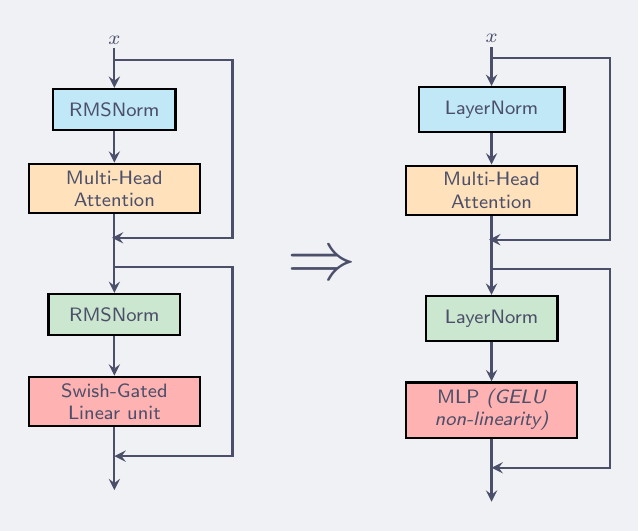
\begin{tikzpicture}[RIR/.style={draw=black,thick,rectangle},AR/.style={->,thick,>=stealth}]
        \scriptsize 
        % RMS Pre-Normalization
        \node[RIR,fill=sblue,inner sep=5pt] (prenorm) {\parbox{1.2cm}{\centering RMSNorm}};
        % MHA Block (Abstracted as already iimplemented)
        \node[RIR,fill=sorange,anchor=north] (mha) at ($(prenorm.south)+(0,-0.4)$) {
            \parbox{2cm}{\centering Multi-Head Attention
            }};
        % Add the Attention Output and the original Input
        \draw[<-,thick,>=stealth] (prenorm.north) -- node[name=fromx,pos=0.65,inner sep=0pt]{} ++ (0,0.5) node[pos=1.2]{$x$};
        % Implement the RMS Again
        \node[RIR,anchor=north,fill=sgreen, inner ysep=5pt] (prermsffn) at ($(mha.south)+(0,-1)$) {
            \parbox{1.5cm}{\centering RMSNorm}
            };
        % FFN after the normalization
        \node[RIR,fill=red!30,anchor=north] (L1) at ($(prermsffn.south)+(0,-0.5)$) {\parbox{2cm}{\centering Swish-Gated Linear unit}};
        % ARRROWS 
        % PreNorm to MHA
        \draw[AR] (prenorm.south) -- (mha.north);
        % MHA to FFN VIA RMS NORM AGAIN
        \draw[AR] (mha.south) -- node[pos=0.3,name=conc1,inner sep=0]{} node[pos=0.7,name=conc2,inner sep=0]{} (prermsffn.north);
        \draw[->,thick,>=stealth] (fromx.north) -- ++ (1.5,0) |- (conc1.west);
        \draw[AR] (prermsffn.south) -- node[pos=0.8,inner sep=0pt,name=midtoir]{} (L1.north);
        % L1 TO OUT
        \draw[AR] (L1.south) -- node[pos=0.5,inner sep=0,name=conc3]{} ++ (0,-0.8);
        % RMS AGAIN TO OUT
        \draw[AR] (conc2.north) --++ (1.5,0) |- (conc3.north);
        % ARROW CHANGE TO 
        \node[anchor=west] at ($(mha.east)+(1,-1)$) {\Huge $\Rightarrow$};
        % SECOND ONE FOR VIT
        % LayerNorm1
        \node[RIR,fill=sblue,inner sep=5pt] (prenorm) at ($(prenorm.east)+(4,0)$) {\parbox{1.5cm}{\centering LayerNorm}};
        % MHA Block (Abstracted as already iimplemented)
        \node[RIR,fill=sorange,anchor=north] (mha) at ($(prenorm.south)+(0,-0.4)$) {
            \parbox{2cm}{\centering Multi-Head Attention
            }};
        % Add the Attention Output and the original Input
        \draw[<-,thick,>=stealth] (prenorm.north) -- node[name=fromx,pos=0.65,inner sep=0pt]{} ++ (0,0.5) node[pos=1.2]{$x$};
        % Implement the RMS Again
        \node[RIR,anchor=north,fill=sgreen, inner ysep=5pt] (prermsffn) at ($(mha.south)+(0,-1)$) {
            \parbox{1.5cm}{\centering LayerNorm}
            };
        % FFN after the normalization
        \node[RIR,fill=red!30,anchor=north] (L1) at ($(prermsffn.south)+(0,-0.5)$) {\parbox{2cm}{\centering MLP \it (GELU\\non-linearity)}};
        % ARRROWS 
        % PreNorm to MHA
        \draw[AR] (prenorm.south) -- (mha.north);
        % MHA to FFN VIA RMS NORM AGAIN
        \draw[AR] (mha.south) -- node[pos=0.3,name=conc1,inner sep=0]{} node[pos=0.7,name=conc2,inner sep=0]{} (prermsffn.north);
        \draw[->,thick,>=stealth] (fromx.north) -- ++ (1.5,0) |- (conc1.west);
        \draw[AR] (prermsffn.south) -- node[pos=0.8,inner sep=0pt,name=midtoir]{} (L1.north);
        % L1 TO OUT
        \draw[AR] (L1.south) -- node[pos=0.5,inner sep=0,name=conc3]{} ++ (0,-0.8);
        % RMS AGAIN TO OUT
        \draw[AR] (conc2.north) --++ (1.5,0) |- (conc3.north);
    \end{tikzpicture}
\end{figure}
\end{minipage}%
\hspace{25pt}
\begin{minipage}[t]{.4\textwidth}
  \raggedright
  \scriptsize 
\end{minipage}
\end{figure}
% ==================================================
\pagebreak
% PAGE 22
\begin{figure}[!htb]
    \begin{minipage}[t]{0.65\textwidth}
    \raggedright
    \customtext{xtitle}{0em}{Understanding the image embeddings for ViT}\\
    Going onto the interesting part of what makes this pioneering research awesome, 
    is how the image patches is handled.
    As described in {\it page 3 section 3.1} of the paper\sidecite{33},
    % \vspace{1em}\\
    {\it\small we reshape the image $\text{x}\in R^{H\times W\times C}$ into a 
    sequence of flattened 2D patches $\text{x}_p\in R^{N\times (P^2\cdot C)}$,
    where $(H,W)$ is the resolution of the original image, $C$ is the number 
    of channels, $(P,P)$ is the resolution of each image patch, and $N = HW/P^2$ 
    is the resulting number of patches, which also serves as the effective 
    input sequence length for the Transformer.}
    \vspace{0.5em}\\
    Let's implement this process in three ways
    \begin{itemize}[left=0pt,topsep=0pt,itemsep=-1ex,parsep=0ex]
        \item using torch unfold
        \item using einops Rearrange
        \item using torch convolution
      \end{itemize}
      \vspace{1em}
      \customtitle{torch unfold}
      PyTorch is an awesome framework, and with it comes one nice functionality, 
      {\it torch unfold}{\maincitecount}, the functionality behind the very core 
      convolution operations in convolutional neural networks. So how does it work?\\
      Imagine we have a 3-channel tensor, then {\it unfold} extracts the patch of a given 
      kernel size across all channels in the tensor and unrolls it to a single column, 
      before proceeding to the next patch as noted by the stride\maincitecount.
\begin{figure}[H]
    \tikzset{matrixlayer/.style={
    matrix of math nodes,nodes in empty cells,
    nodes={draw=#1,fill=#1!15,minimum size=4mm,anchor=center,text=black},
    column sep=-.1*\pgflinewidth,
    row sep=-.1*\pgflinewidth
    }}
    \begin{tikzpicture}[>=stealth,AR/.style={>=stealth,->,thick}]
        \tiny
        \begin{scope}[shift={(45:2)}]
        \node[matrixlayer=red] (m3){
        32& 33 & 34 & 35 \\
        36& 37 & 38 & 39 \\
        40 & 41 & 42 & 43 \\
        44 & 45 & 46 & 47\\
        };
        \end{scope}
        \begin{scope}[shift={(45:1)},opacity=0.75]
        \node[matrixlayer=teal] (m2){
        16 & 17 & 18 & 19 \\
        20 & 21 & 22 & 23 \\
        24 & 25 & 26 & 27 \\
        28 & 29 & 30 & 31 \\
        };
        \end{scope}
        \begin{scope}[opacity=0.75]
        \node[matrixlayer=blue] (m1){
        0 & 1 & 2 & 3 \\
        4 & 5 & 6 & 7 \\
        8 & 9 & 10 & 11 \\
        12 & 13 & 14 & 15 \\
        };
        \end{scope}
        \begin{scope}[->,thick]
        \draw ([shift={(0,-.3)}]m1.south west)--([shift={(0,-.3)}]m1.south east) node[midway,below]{$W$};
        \draw ([shift={(.0,0)}]m1.south east)--([shift={(.0,0)}]m3.south east) node[midway,below,rotate=45]{$C$};
        \draw ([shift={(-.3,0)}]m1.north west)--([shift={(-.3,0)}]m1.south west) node[midway,left]{$H$};
        \end{scope}
        \node (unfoldcode) at ($(m1.south east)+(2.7,0)$){\usebox{\unfold}};
        \draw[AR]($(m3.east)$) -- node[below]{\scriptsize unfold\maincitecount} ++ (3,0) node[pos=1.2,matrixlayer=spurple,anchor=west]{        
        0 & 2 & 8 & 10 \\
        1 & 3 & 9 & 11 \\
        4 & 6 & 12 & 14 \\
        5 & 7 & 13 & 15 \\
        16 & 18 & 24 & 26 \\
        17 & 19 & 25 & 27 \\
        20 & 22 & 28 & 30 \\
        21 & 23 & 29 & 31 \\
        32 & 34 & 40 & 42 \\
        33 & 35 & 41 & 43 \\
        36 & 38 & 44 & 46 \\
        37 & 39 & 45 & 47 \\
        };
        \draw[AR,red] ($(unfoldcode.north)+(.3,0)$) --++(0,1);
        \end{tikzpicture}\\
    Next, let's create patches from an image and visualize them for the different kernel sizes. 
    Let's consider this image I once used in the {\it From Tensors to Residual Learning}\maincitecount 
    course which I taught in PyTorch and focused on the fundamentals of Deep Learning from the 
    mathematics of Calculus to implementing the different variants of residual network architectures.
\end{figure}
% \begin{lstlisting}[language=python,style=python,basicstyle=\ttfamily\footnotesize]
% \end{lstlisting}
\end{minipage}%
\hspace{25pt}
\begin{minipage}[t]{.4\textwidth}
  \raggedright
  \scriptsize 
  \sidecitecount \href{https://docs.pytorch.org/docs/stable/generated/torch.nn.Unfold.html}{Unfold}\\
    PyTorch API reference
    \vspace{2em}\\
    \sidecitecount the tensor needs extrusion to the batch dimension since unfold only supports 4-D tensors
    \vspace{2em}\\
    \sidecitecount Note that {\it unfold} gives us the flattened 2D patches as a transpose of the expected 2D patches 
    in the paper, since we have in the resulting visual  $(P^2\cdot C)\times N$ when we need its transpose, denoted 
    as $\text{x}_p$ in the paper of dims $N\times(P^2\cdot C)$. This will be handy later on!
    \vspace{2em}\\
    \sidecitecount \href{https://youcanjustbuild.com/courses/fromtensorstoresidual}{\it From Tensors To Residual Learning}\\
    {\it From the math of tensors to the implementation\\of residual learning}
\end{minipage}
\end{figure}
% ==================================================
\pagebreak
% PAGE 23
\begin{figure}[!htb]
    \begin{minipage}[t]{0.65\textwidth}
    \raggedright
    Huggingface datasets\includegraphics[width=0.05\textwidth]{images/hf-logo.png} come in handy for this, getting the image 
    which is a \textit{Pillow} instance which we then transform to a {\it torch Tensor}
\begin{lstlisting}[language=python,style=python,basicstyle=\ttfamily\footnotesize]
from datasets import load_dataset
from  torchvision.transforms.v2.functional import (
    pil_to_tensor, resize)
# function to resize the image to 240 by 240
resize_fn = lambda x, size=240: resize(
    x, size=[size,size]).to(torch.float32)

dataset = load_dataset("huggingface/cats-image")
image = dataset['test']['image'][0]
image = pil_to_tensor(image)
image = resize_fn(image)
C,H,W=image.shape
\end{lstlisting}
Let's of course initialize the unfold instance. We want to get, for now, 4 patches
from the image, this means the patch size is
\vspace{-1em}
$$N=HW/P^2\Rightarrow 4=(240/P)^2\Rightarrow P=120$$
\vspace{-2em}
\begin{lstlisting}[language=python,style=python,basicstyle=\ttfamily\footnotesize]
P=120
unfold = nn.Unfold(kernel_size=(P, P),stride=P)
patches = unfold(image)
print(patches.shape) # torch.Size([1, 43200, 4])
\end{lstlisting}
and so the patches can be converted to images as 
\begin{lstlisting}[language=python,style=python,basicstyle=\ttfamily\footnotesize]
def extractPatch(patches, index, P):
    patch = patches[...,index].view(1,3,P,P)
    patch = patch.squeeze(0).permute(1,2,0)
    return patch.to(torch.uint8).numpy()
\end{lstlisting}
and visualize\maincitecount\ the image patches using the code 
\begin{lstlisting}[language=python,style=python,basicstyle=\ttfamily\footnotesize]
showPatches(patches,N,P)
\end{lstlisting}
to get
\vspace{-1.8em}
\begin{figure}[H]
    \centering
    \includegraphics[width=.6\textwidth]{images/image-patches.png}
\end{figure}
\end{minipage}%
\hspace{25pt}
\begin{minipage}[t]{.4\textwidth}
  \raggedright
  \scriptsize 
  \sidecitecount 
\begin{lstlisting}[language=python,style=python,basicstyle=\ttfamily\tiny]
import matplotlib.pyplot as plt

def showPatches(patches, N, P):
    rows=cols=int(N**.5)
    for i in range(N):
        plt.subplot(rows,cols,i+1)
        patch_image = extractPatch(patches, i, P)
        plt.imshow(
            patch_image,aspect = "auto"
            )
        plt.tight_layout()
        plt.xticks([]); plt.yticks([])
    plt.subplots_adjust(
    hspace=0.1,wspace=0.1 # wspace => aspect auto
    )
    plt.show()
\end{lstlisting}
\end{minipage}
\end{figure}
% ==================================================
\pagebreak
% PAGE 24
\begin{figure}[!htb]
    \begin{minipage}[t]{0.65\textwidth}
    \raggedright
    \customtext{xtitle}{0em}{The next big thing, einops\maincitecount}\\
    This library greatly simplifies a lot of incredible operations, and is 
    greatly used even in simplifying high dimensional matrix-multiplication 
    heavy layers in many model graphs.\\
    The docs is wonderful and on the side notes for in-depth review. 
    In this case, we want to get the image dimensions, and then get the 
    height and width as integer multiples of the patch size, but we need to 
    be cautious on how we handle the channel dimensions, that is, how we translate 
    the unfold operation as either channel dimensions first or spatial dimensions
    first.
    This change in dimensions is implemented using einops as     
\begin{lstlisting}[language=python,style=python,basicstyle=\ttfamily\footnotesize]
from einops.layers.torch import Rearrange
rearr = Rearrange(
    'b c (h p1) (w p2) -> b (c p1 p2) (h w)', 
    p1 = P, p2 = P)
\end{lstlisting}
considering that the image is already a {4D} tensor. The above operations says,
hey, let's take subsets of the spatial dimensions across all channels, then 
rearrange the dimensions to a batch of these tensors of size {\small$P^2\cdot C$},
$N$ of such. Reminder that this is the transpose of $x_p$.
It can be invoked to get the image patches as below which then gives the 
same results as the visual just above.
\begin{lstlisting}[language=python,style=python,basicstyle=\ttfamily\footnotesize]
patches_again = rearr(image)
showPatches(patches_again,N,P)
\end{lstlisting}
\customtitle{using torch convolution}
I've always loved convolution, because I love signal processing, and I love image processing,
and I love Computer Vision. And convolution, this operation, is core in many topics across 
these domains.\\
Convolution neural networks is inspired by the biological cortex and I've gone through it in-depth 
in my course\maincitecount.
\begin{figure}[H]
    \begin{tikzpicture}[
    RIR/.style={draw=black, very thick, rectangle, rounded corners, inner sep=5pt, inner ysep=5pt},
    AR/.style={>=stealth,thick,->}
    ]
    % \begin{scope}[shift={(45:1.5)}]
    % \node[RIR,fill=sgreen] (m3){
    % hello
    % };
    % \end{scope}
    % \begin{scope}[shift={(45:1)}]
    % \node[RIR,fill=sorange] (m2){
    % hello
    % };
    % \end{scope}
    % \begin{scope}[shift={(45:0)}]
    % \node[RIR,fill=spurple] (m1){
    % hello
    % };
    % \end{scope}
    \def\colors{sgreen,spurple,sorange,syellow,sblue,sstart}
        % \foreach \Z in {0,0.5,1,1.5}
        %     {\draw[fill=red,draw=red!10] (-1,-1,\Z) rectangle (2,2,\Z);}
        \foreach \color [count=\i from 0] in \colors {
        \def\j{\i*.5}
        %\StrBehind{\color}{s}[\hello]
        %\draw[fill=\color,draw=\hello,thick,rounded corners=2pt] (-1,-1,\j) rectangle (2,2,\j);
        \draw[fill=\color,draw=black,thick,rounded corners=2pt] (-0.5,-0.5,\j) rectangle (0.5,0.5,\j);
        \ifnum\i=2\breakforeach\fi
        }
        \draw[AR,<->](0,-1.15) -- node[midway,below,rotate=40]{
        \fontsize{5}{4}\selectfont \bf 3 channels
        } ++ (0.7,0.6);
        \draw[AR,<->](0,-1.15) -- node[midway,below]{\tiny 4} ++ (-0.8,0);
        \draw[AR,<->](-1.1,-0.8) -- node[midway,left]{\tiny 4} ++ (0,0.8);
        \node[red] at (-0.5,-1.8) {\usebox{\convimage}};
        \node[red] at (6.5,-1.8) {\usebox{\convkernels}};

        \def\colors{syellow,sblue,sstart}          
        \begin{scope}[shift={(4.5, 1, 0)}]
        \foreach \color [count=\i from 0] in \colors {
        \def\j{\i*.3}
        \node[draw=black, fill=\color, thick, rounded corners=2pt, minimum width=1cm, minimum height=1cm] 
            at (0, 0, \j) (kerns-\i) {};
        \ifnum\i=2\breakforeach\fi
        }
        \node[RIR,fill=sorange,draw=black,thin,rounded corners=0,inner sep=2pt] 
        at ($(kerns-1.south)+(0,-0.5)$){\tiny bias};
        \end{scope}
        \begin{scope}[shift={(3.5, 0, 0)}]
        \foreach \color [count=\i from 0] in \colors {
        \def\j{\i*.3}
        \node[draw=black, fill=\color, thick, rounded corners=2pt, minimum width=1cm, minimum height=1cm] 
            at (0, 0, \j) (kerns-\i) {};
        \ifnum\i=2\breakforeach\fi
        }
        \node[RIR,fill=sorange,draw=black,thin,rounded corners=0,inner sep=2pt] 
        at ($(kerns-1.south)+(0,-0.5)$){\tiny bias};
        \end{scope}
        \begin{scope}[shift={(2.5, -1, 0)}]
        \foreach \color [count=\i from 0] in \colors {
        \def\j{\i*.3}
        % \draw[fill=\color,draw=black,thick,rounded corners=2pt] (-0.5,-0.5,\j) rectangle (0.5,0.5,\j);
        \node[draw=black, fill=\color, thick, rounded corners=2pt, minimum width=1cm, minimum height=1cm] 
            at (0, 0, \j) (kerns-\i) {};
        \ifnum\i=2\breakforeach\fi
        }
        \draw [decorate,decoration={brace,mirror,raise=4ex},red] (-0.2,-0.3) -- (0.2,0) node[yshift=-2em,xshift=1.5em,midway,rotate=40] {\tiny filter};
        \node[RIR,fill=sorange,draw=black,thin,rounded corners=0,inner sep=2pt] 
        at ($(kerns-1.south)+(0,-0.5)$){\tiny bias};
        \draw [AR,red!70] ($(kerns-0.south)+(-0.9,-0.9)$) 
        node[below,inner sep=0]{\tiny kernel} to 
        [out=80,in=-90] ($(kerns-0.south)+(-0.3,-0.2)$);
        \end{scope}
        % OUTPUT
        \begin{scope}[shift={(7.5, 0.5, 0)}]
    \def\colors{spurple,sorange,sblue}
        \foreach \color [count=\i from 0] in \colors {
        \def\j{\i*.3}
        % \draw[fill=\color,draw=black,thick,rounded corners=2pt] (-0.5,-0.5,\j) rectangle (0.5,0.5,\j);
        \node[draw=black, fill=\color, thick, rounded corners=2pt, minimum width=1cm, minimum height=1cm] 
            at (0, 0, \j) (kerns-\i) {};
        \ifnum\i=2\breakforeach\fi
        }
        \node[anchor=west] at ($(kerns-2.east)+(0.4,0.5)$) {
            \parbox{5cm}{
                \tiny \it output size\vspace{0.3em}\\
                $\Big\lfloor \frac{n+2p-f}{s}+1\Big\rfloor$\\
                $\Big\lfloor \frac{4+0-2}{1}+1\Big\rfloor$
                \vspace{0.3em}\\
                output size is 3
            }
        };
        \end{scope}
    \end{tikzpicture}
\end{figure}
\end{minipage}%
\hspace{25pt}
\begin{minipage}[t]{.4\textwidth}
  \raggedright
  \scriptsize 
  \sidecitecount \url{https://einops.rocks/pytorch-examples.html}\\
  {\it Writing a better code with pytorch and einops}
  \vspace{2em}\\
  \sidecitecount \url{https://youcanjustbuild.com/courses/from-tensors-to-residual-learning/foundations}\\
  {\it The foundations of residual learning}
\end{minipage}
\end{figure}
% ==================================================
\pagebreak
% PAGE ###
\begin{figure}[!htb]
\begin{minipage}[t]{0.65\textwidth}
\raggedright
Using convolution to get the image patches, the kernel size will be the size of the 
needed patch with the stride being the same, the output channels becomes D.
\begin{lstlisting}[language=python,style=python,basicstyle=\ttfamily\footnotesize]
patch_layer=nn.Conv2d(3, 768, kernel_size=(16, 16), stride=(16, 16))
\end{lstlisting}
\customtitle{Now onto implementing the image embeddings}
Note that as we understood from the side note\sidecite{38}, we have to transpose 
how we actually got the patches to 
\begin{lstlisting}[language=python,style=python,basicstyle=\ttfamily\footnotesize]
    Rearrange('b c (h p1) (w p2) -> b (h w) (p1 p2 c)',
            p1=P,p2=P)
\end{lstlisting}
which then gives us the {2D} flattened patches 
{\footnotesize $x_p\in R^{N\times(P^2\cdot C)}$}
The layers that hence map the patches to the D dimensions linearly to give the
{\it \color{xtitle} patch embeddings} is 
constructed as\maincitecount
\begin{lstlisting}[language=python,style=python,basicstyle=\ttfamily\footnotesize]
patches_layer = nn.Sequential(
    Rearrange('b c (h p1) (w p2) -> b (h w) (p1 p2 c)',
    p1 = P, p2 = P),
    nn.LayerNorm(patch_dim),
    nn.Linear(patch_dim,dim))
\end{lstlisting}    
we then neeed to prepend a class token\maincitecount\ to the sequence of embedded patches\\
$[\text{x}_{\text{class}};\text{x}_p^1\text{\bf E};\text{x}_p^2\text{\bf E};\cdots;\text{x}_p^N\text{\bf E}]$
\begin{lstlisting}[language=python,style=python,basicstyle=\ttfamily\footnotesize]
patch_embs = patches_layer(image)
cls_token = nn.Parameter(torch.randn(1, 1, dim))
x = torch.cat((cls_token,patch_embs),dim=1)
\end{lstlisting}
\customtext{xtitle}{0em}{Adding positional embeddings to the patch embeddings}\\
By simplifying their learning embedding from the advanced 2D-aware position 
embedding due to no significant performance, the paper uses 1D position embeddings
defined by {\small $E_{pos}\in R^{(N+1)\times D}$}.
\begin{lstlisting}[language=python,style=python,basicstyle=\ttfamily\footnotesize]
position_embeddings = nn.Parameter(
    torch.randn(1,N+1,dim))
\end{lstlisting}
and now we add the resulting embedding to the positional embedding
\begin{lstlisting}[language=python,style=python,basicstyle=\ttfamily\footnotesize]
x += pos_embeddings[:,(N+1)]
\end{lstlisting}
and that is it to give us the whole implementation as 
\end{minipage}%
\hspace{25pt}
\begin{minipage}[t]{.4\textwidth}
  \raggedright
  \scriptsize 
  \sidecitecount the original ViT uses image resized to 256 with patch size of 
  16 and D being 768 for {\it ViT-Base 16}. {\it patch\_dim} is basically $C\times P^2$.
  \vspace{2em}\\
  \sidecitecount In the interesting implementing of {\it Vision Transformers},
  some {\it 10x} engineers opted for toggling between mean pooling and cls tokens 
  computed with the original patch embeddings. You can see their awesome implementation 
  of such in their codebase\\ 
  \url{https://github.com/lucidrains/vit-pytorch/blob/main/vit_pytorch/vit.py}
\end{minipage}
\end{figure}
% ==================================================
\pagebreak
% PAGE ###
\begin{figure}[!htb]
    \begin{minipage}[t]{0.65\textwidth}
    \raggedright
    \customtext{xtitle}{0em}{The next big thing, einops}\\
\begin{lstlisting}[language=python,style=python,basicstyle=\ttfamily\footnotesize]
class ImageEmbeddings(nn.Module):
    def __init__(self, H, W, C, P, dim):
        super(ImageEmbeddings,self).__init__()
        N = int((H*W)/(P**2)); self.N = N
        assert H%N==0 and W%N==0, \
            "image size must be integer multiple of patch"
        patch_dim = C*P**2
        self.patch_layers = nn.Sequential(
            Rearrange(
            'b c (h p1) (w p2) -> b (h w) (p1 p2 c)', 
            p1 = P, p2 = P),
            nn.LayerNorm(patch_dim),
            nn.Linear(patch_dim,dim),
        )
        self.class_tokens = nn.Parameter(torch.randn(1, 1, dim))
        self.position_embeddings = nn.Parameter(torch.randn(1,N+1,dim))
    def forward(self,image):
        x = self.patch_layers(image)
        x = torch.cat((self.class_tokens,x),dim=1)
        return += self.position_embeddings[:,:(self.N+1)]
\end{lstlisting}
% \begin{lstlisting}[language=python,style=python,basicstyle=\ttfamily\footnotesize]
% \end{lstlisting}
\end{minipage}%
\hspace{25pt}
\begin{minipage}[t]{.4\textwidth}
  \raggedright
  \scriptsize 
\end{minipage}
\end{figure}
% ==================================================
\end{document}

